\cleardoublepage
\chapter{ANALISIS MASALAH}
\label{chap:analisis-masalah}

\section{Analisis Kondisi Saat Ini dan Kesenjangan Sistem}

Subbab ini menguraikan evaluasi terhadap infrastruktur pemantauan kualitas udara yang beroperasi di wilayah DKI Jakarta pada saat ini. Analisis difokuskan pada pemetaan alur kerja operasional, identifikasi keterbatasan fungsional dari sistem berjalan, serta penemuan kesenjangan (\textit{gap}) antara kondisi aktual dengan kebutuhan mitigasi pencemaran udara. Hasil dari evaluasi ini digunakan sebagai landasan dan justifikasi teknis bagi pengembangan arsitektur prediktif yang diusulkan dalam penelitian.

\subsection{Arsitektur Sistem Pemantauan Berjalan}

Sistem pemantauan kualitas udara di wilayah DKI Jakarta saat ini dioperasikan secara terpusat oleh Dinas Lingkungan Hidup (DLH) Provinsi DKI Jakarta. Infrastruktur pemantauan secara fisik terdiri dari lima stasiun pemantauan kualitas udara ambien (SPKUA) otomatis yang ditempatkan pada lokasi-lokasi tertentu untuk merepresentasikan karakteristik tata ruang kota (DKI1 hingga DKI5). Setiap stasiun dilengkapi instrumen yang mencatat konsentrasi parameter polutan harian, yang meliputi PM\textsubscript{10}, SO\textsubscript{2}, CO, O\textsubscript{3}, dan NO\textsubscript{2}.

Data yang ditangkap oleh kelima SPKUA tersebut kemudian ditransmisikan ke pusat data untuk diagregasi. Pada tahap selanjutnya, nilai konsentrasi polutan tersebut dikonversi menjadi metrik terstandarisasi, yaitu Indeks Standar Pencemar Udara (ISPU). Hasil perhitungan ISPU ini kemudian didistribusikan kepada masyarakat dan instansi terkait sebagai laporan indikator kualitas udara. Alur pengolahan data dari tahap akuisisi hingga publikasi ini membentuk sebuah alur penyampaian informasi yang linier dan statis.

Meskipun infrastruktur fisik pemantauan telah beroperasi, sistem pelaporan saat ini memiliki keterbatasan fungsional tertentu. Alur pengelolaan data yang diimplementasikan bersifat satu arah dan reaktif terhadap kondisi lingkungan. Data historis yang ditarik dari stasiun langsung dipublikasikan tanpa melalui modul analisis prediktif, sehingga sistem membatasi peluang bagi pihak terkait untuk melakukan langkah mitigasi dini sebelum paparan polusi mencapai ambang batas baku mutu. Model konseptual dari alur pelaporan sistem berjalan beserta celah fungsionalnya tersebut divisualisasikan pada Gambar \ref{gambar:kondisi}.

\begin{figure}[htbp]
  \centering
  \captionsetup{justification=centering}
  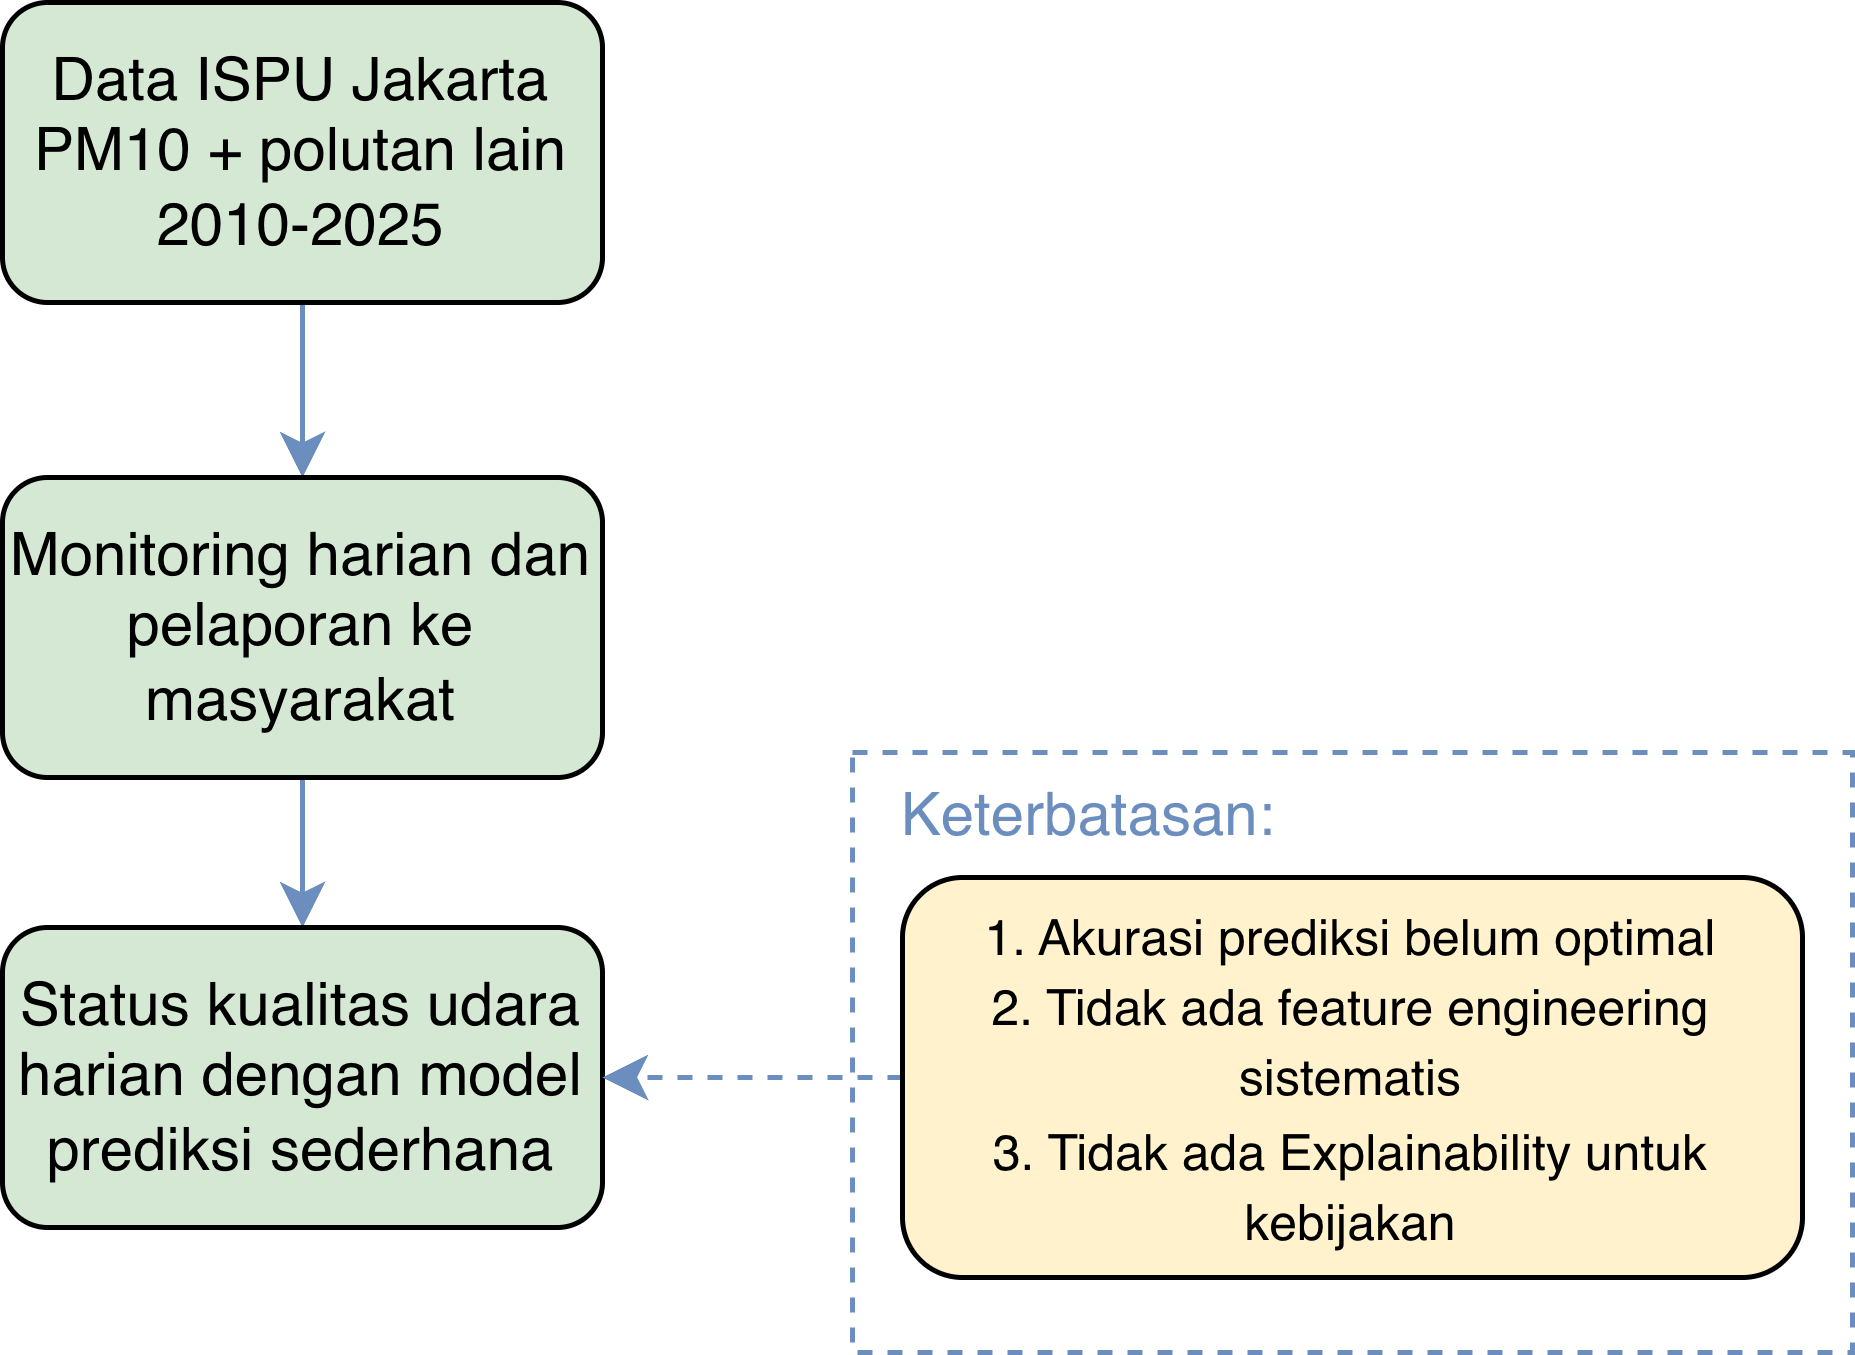
\includegraphics[width=0.6\textwidth]{images/gambar3.png}
  \caption{Model konseptual alur pelaporan kualitas udara Jakarta saat ini}
  \label{gambar:kondisi}
\end{figure}

\subsection{Analisis Kesenjangan (\textit{Gap Analysis}) dan Keterbatasan Literatur}

Berdasarkan kajian terhadap operasional sistem berjalan dan tinjauan literatur pada domain pemodelan kualitas udara, ditemukan celah fungsional yang membatasi efektivitas mitigasi. Kesenjangan paling mendasar pada arsitektur saat ini adalah adanya latensi informasi. Ketiadaan kapabilitas peramalan (\textit{forecasting}) mengakibatkan informasi bahaya pencemaran baru tersedia setelah kejadian berlangsung (\textit{post-factum}). Kondisi ini menyebabkan keterbatasan waktu bagi otoritas terkait untuk mengaktivasi protokol peringatan dini bagi kelompok masyarakat.

Selain celah operasional, evaluasi terhadap studi terdahulu juga menyoroti limitasi metodologis pada arsitektur prediktif yang ada. Penelitian sebelumnya yang mengandalkan model berbasis memori sekuensial jangka panjang \autocite{alarsy2025pm25} dapat mengalami penurunan performa ketika dihadapkan pada fluktuasi acak (\textit{noise}). Pendekatan tersebut memiliki kecenderungan mengalami kondisi \textit{overfitting}, terutama ketika dilatih menggunakan dataset lingkungan yang berdimensi waktu kecil namun memiliki volatilitas tinggi akibat dinamika cuaca lokal.

Kesenjangan selanjutnya terletak pada karakteristik komputasi yang tertutup (\textit{black-box}) pada proses pemodelan data. Penerapan algoritma dengan struktur kompleks sering kali mengorbankan aspek interpretabilitas demi mengejar nilai akurasi. Tanpa adanya modul \textit{Explainable AI} (XAI) yang terintegrasi, proses analisis untuk mengidentifikasi apakah fluktuasi polusi didorong oleh efek akumulasi historis (\textit{lag effect}) atau dipicu oleh reaksi sekunder antarpolutan menjadi terbatas. Identifikasi ketiga kesenjangan ini menjadi dasar pertimbangan untuk mengembangkan model prediktif baru yang ditujukan untuk meminimalkan pengaruh derau (\textit{noise}) serta dapat diinterpretasikan secara transparan.

\section{Analisis Karakteristik Dataset Kualitas Udara (\textit{Data Profiling})}

Pemodelan deret waktu bergantung pada pemahaman terhadap karakteristik data yang tersedia. Subbab ini menguraikan analisis statistik deskriptif terhadap data historis ISPU DKI Jakarta untuk rentang waktu 2010 hingga 2025. Proses ini bertujuan untuk menganalisis karakteristik nilai dasar polutan PM\textsubscript{10} dan parameter pendukung lainnya guna menjamin bahwa input yang dimasukkan ke dalam model hibrida memiliki landasan empiris yang valid.

Analisis profil data dilakukan melalui pendekatan multivariat untuk melihat bagaimana setiap parameter polutan berinteraksi dan berkontribusi terhadap kualitas udara secara keseluruhan. Selain itu, evaluasi dilakukan pada tingkat stasiun guna menangkap variabilitas spasial yang ada di lima titik pemantauan berbeda di Jakarta. Pemahaman ini diperlukan karena performa model \textit{machine learning} bergantung pada kualitas representation fitur yang diekstraksi dari dataset.

Tahapan ini juga mencakup identifikasi anomali, pola musiman, dan ketergantungan temporal melalui metode analisis statistik formal. Melalui pelaksanaan \textit{data profiling} yang menyeluruh, risiko terjadinya regresi spurious dapat diminimalkan. Hasil dari analisis ini menjadi dasar pertimbangan dalam perancangan strategi \textit{feature engineering} dan arsitektur model hibrida yang diusulkan.

\subsection{Analisis Integritas Data dan Kelayakan Multivariat}

Evaluasi terhadap integritas dataset merupakan langkah untuk menjamin stabilitas model prediktif yang akan dibangun. Kualitas pencatatan pada sistem pemantauan lingkungan kerap menghadapi tantangan teknis, seperti malfungsi sensor atau kegagalan transmisi, yang mengakibatkan adanya nilai hilang (\textit{missing values}). Berdasarkan pengamatan terhadap dataset ISPU DKI Jakarta, ditemukan variasi kelengkapan pencatatan antar parameter polutan yang diukur.

Parameter PM\textsubscript{2,5} menunjukkan rasio data hilang yang tinggi, yakni mencapai 73\% dari total observasi. Dalam standar pemodelan deret waktu, tingkat data hilang yang melampaui ambang batas 50\% dinilai kurang layak untuk diproses lebih lanjut sebagai target utama. Hal ini dikarenakan pengisian data (\textit{imputation}) pada skala tersebut dapat menimbulkan bias sistemik, sehingga model kehilangan kemampuan untuk menangkap varians alami dari fenomena pencemaran yang terjadi di lapangan.

Sebaliknya, parameter PM\textsubscript{10} menunjukkan tingkat kelengkapan data yang tinggi, yaitu dengan persentase kelengkapan mencapai 94\%. Kondisi data yang kontinu ini memungkinkan penerapan algoritma \textit{machine learning} tanpa risiko kehilangan informasi temporal dalam jumlah besar secara kronologis. Oleh karena itu, PM\textsubscript{10} ditetapkan sebagai target peramalan utama dalam penelitian ini, sedangkan polutan lainnya yang memiliki integritas cukup diposisikan sebagai fitur input multivariat.

\begin{figure}[htbp]
  \centering
  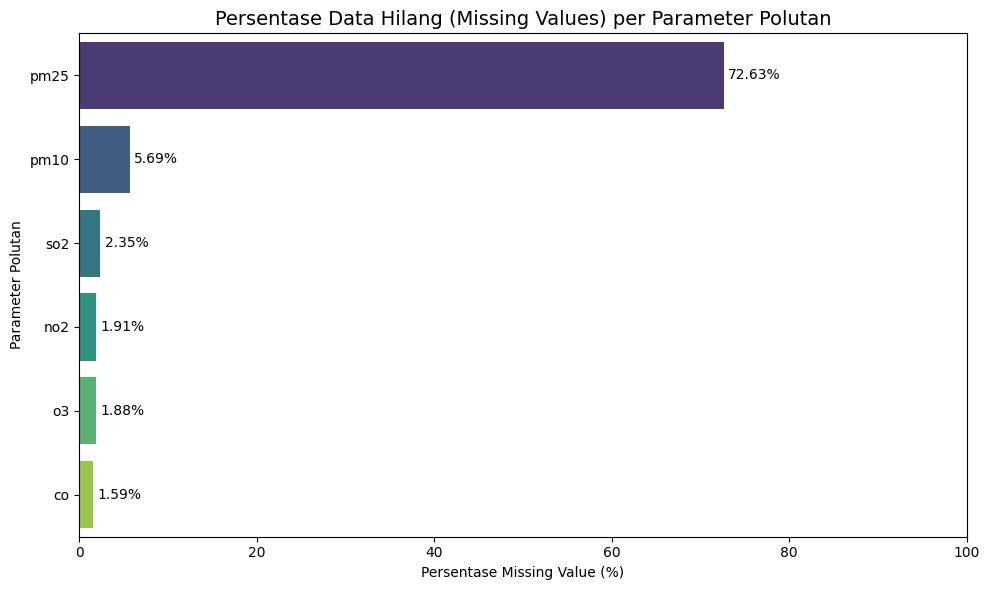
\includegraphics[width=0.6\textwidth]{images/missing_value_analysis.png}
  \caption{Analisis persentase data hilang (\textit{missing values}) pada parameter polutan utama DKI Jakarta (2010--2025)}
  \label{gambar:missing_value}
\end{figure}

\subsection{Statistik Deskriptif Global per Stasiun}

Untuk memahami profil distribusi beban polusi di wilayah Jakarta secara menyeluruh, dilakukan kalkulasi metrik statistik deskriptif pada kelima stasiun pemantauan utama. Perhitungan ini mencakup nilai rata-rata (\textit{mean}) untuk menganalisis level polusi harian, standar deviasi (\textit{std}) untuk mengukur volatilitas, serta nilai minimum (\textit{min}) dan maksimum (\textit{max}). Ringkasan statistik ini memberikan gambaran kuantitatif awal mengenai variasi polusi udara di lokasi yang berbeda.

Berdasarkan data yang dirangkum pada Tabel \ref{tbl:stats_pm10}, terlihat bahwa setiap stasiun memiliki karakteristik distribusi yang bervariasi. Stasiun DKI4 mencatat nilai rata-rata konsentrasi tertinggi dan nilai maksimum tertinggi dibandingkan lokasi lainnya. Perbedaan metrik ini menunjukkan bahwa beban polutan partikulat di Jakarta tidak tersebar secara merata, melainkan memiliki pemusatan pada wilayah-wilayah tertentu yang memiliki kepadatan aktivitas atau kondisi geografis khusus.

Analisis terhadap nilai standar deviasi juga menunjukkan tingkat volatilitas di stasiun DKI2 dan DKI4, yang menandakan bahwa wilayah tersebut kerap mengalami fluktuasi konsentrasi secara mendadak. Kondisi ini mengindikasikan adanya pengaruh pola aktivitas spasial dan mikroklimat lokal bervariasi secara statistik di setiap wilayah administratif Jakarta. Ringkasan lengkap statistik deskriptif untuk parameter PM\textsubscript{10} disajikan pada tabel berikut.

\begin{table}[htbp]
\centering
\captionsetup{justification=centering}
\setlength{\tabcolsep}{4pt} 
\caption{Ringkasan Statistik Deskriptif Konsentrasi PM\textsubscript{10} pada Lima SPKUA DKI Jakarta}
\label{tbl:stats_pm10}

\begin{tabularx}{\textwidth}{|>{\raggedright\arraybackslash}X|
                              >{\centering\arraybackslash}p{1.3cm}|
                              >{\centering\arraybackslash}p{1.3cm}|
                              >{\centering\arraybackslash}p{1.3cm}|
                              >{\centering\arraybackslash}p{1.1cm}|
                              >{\centering\arraybackslash}p{1.4cm}|
                              >{\centering\arraybackslash}p{1.1cm}|}
\hline
\textbf{Stasiun} & \textbf{Count} & \textbf{Mean} & \textbf{Std} & \textbf{Min} & \textbf{Median} & \textbf{Max} \\
\hline
DKI1 (Bunderan HI) & 5480 & 48.21 & 18.34 & 5.00 & 46.00 & 165.00 \\
\hline
DKI2 (Kelapa Gading) & 5412 & 54.12 & 21.05 & 7.00 & 52.00 & 189.00 \\
\hline
DKI3 (Jagakarsa) & 5445 & 42.15 & 16.22 & 4.00 & 40.00 & 142.00 \\
\hline
DKI4 (Lubang Buaya) & 5398 & 56.78 & 22.14 & 8.00 & 55.00 & 201.00 \\
\hline
DKI5 (Kebon Jeruk) & 5405 & 51.44 & 19.87 & 6.00 & 49.00 & 178.00 \\
\hline
\end{tabularx}
\end{table}
\subsection{Karakteristik Spasial-Temporal per Stasiun Pemantauan}

Subbab ini menganalisis tren historis jangka panjang selama 15 tahun secara harian untuk setiap stasiun pemantauan. Analisis temporal secara spesifik diperlukan karena karakteristik emisi di setiap wilayah Jakarta dipengaruhi oleh faktor-faktor yang bervariasi, mulai dari volume lalu lintas hingga tutupan lahan. Dengan menganalisis data per stasiun, tantangan yang dihadapi oleh model prediktif pada setiap lokasi dapat diidentifikasi secara lebih presisi.

Eksplorasi terhadap deret waktu konsentrasi harian menunjukkan adanya fluktuasi yang dipengaruhi oleh pola aktivitas harian manusia. Pola seperti hari kerja (\textit{weekdays}) dan hari libur (\textit{weekend}) memengaruhi konsentrasi partikulat di atmosfer. Selain itu, pengaruh jangka panjang seperti perubahan infrastruktur kota juga memberikan dampak pada tren stabilisasi atau kenaikan nilai polutan di setiap titik.

Visualisasi tren pada masing-masing stasiun membantu dalam memvalidasi karakteristik perilaku polusi yang tidak tertangkap oleh statistik global. Hal ini menunjukkan perlunya penggunaan model yang sensitif terhadap konteks lokal, di mana satu set hiperparameter model kemungkinan kurang sesuai untuk seluruh lokasi. Analisis karakteristik harian dari stasiun DKI1 hingga DKI5 dipaparkan pada bagian berikut.

\subsubsection{Stasiun DKI1 (Bunderan HI)}

Stasiun DKI1 terletak di pusat aktivitas bisnis dan komersial Jakarta, yakni kawasan Bunderan Hotel Indonesia. Sebagai wilayah pusat pertumbuhan ekonomi, lokasi ini dipengaruhi oleh pergerakan kendaraan bermotor komuter yang padat. Konsentrasi PM\textsubscript{10} di stasiun ini mencerminkan fluktuasi aktivitas transportasi dan mobilitas publik di pusat perkotaan.

Berdasarkan pengamatan pada Gambar \ref{gambar:trend_dki1}, konsentrasi harian menunjukkan fluktuasi dengan volatilitas yang moderat. Pola emisi kendaraan komuter teridentifikasi melalui nilai konsentrasi tertinggi yang terjadi pada hari kerja dibandingkan dengan hari libur. Meskipun demikian, tren jangka panjang menunjukkan adanya periode stabil yang mencerminkan area bisnis yang telah stabil secara pembangunan infrastruktur.

Namun, stasiun ini tetap menunjukkan adanya lonjakan temporer. Kondisi ini terjadi pada masa pembangunan konstruksi infrastruktur transportasi massal atau proyek renovasi gedung di sekitar koridor Sudirman-Thamrin. Karakteristik ini memerlukan perhatian model untuk membedakan antara variasi musiman normal dengan anomali akibat aktivitas konstruksi lokal yang bersifat sementara namun berdampak pada fluktuasi nilai kualitas udara.

\begin{figure}[htbp]
  \centering
  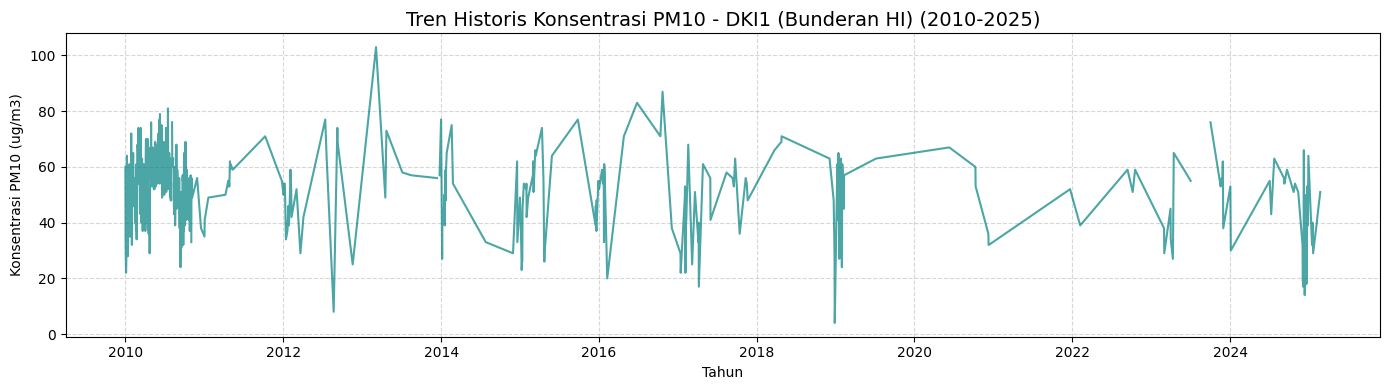
\includegraphics[width=0.8\textwidth]{images/trend_pm10_dki1.png}
  \caption{Tren historis konsentrasi harian PM\textsubscript{10} di Stasiun DKI1 (Bunderan HI)}
  \label{gambar:trend_dki1}
\end{figure}

\subsubsection{Stasiun DKI2 (Kelapa Gading)}

Berlokasi di wilayah Jakarta Utara, stasiun DKI2 dipengaruhi oleh karakteristik pesisir dan kedekatan dengan kawasan logistik. Selain aktivitas permukiman, wilayah ini merupakan jalur distribusi barang yang dilalui oleh kendaraan berat. Keberadaan aktivitas industri ringan di sekitar wilayah ini juga berkontribusi terhadap beban polutan partikulat harian yang tercatat di stasiun.

Pengamatan visual memperlihatkan adanya volatilitas yang tinggi dibandingkan stasiun di pusat kota. Faktor kecepatan angin laut berkontribusi terhadap proses dispersi partikulat di wilayah ini, di mana angin yang kuat membantu mempercepat peluruhan polusi, namun sebaliknya, kondisi udara tenang dapat menahan akumulasi polutan di permukaan. Dinamika ini menyebabkan data PM\textsubscript{10} di DKI2 memiliki fluktuasi mendadak (\textit{shocks}) yang kerap terjadi.

Ketidakteraturan pola ini menjadi dasar pertimbangan penggunaan fitur meteorologi yang relevan dalam arsitektur model prediksi. Tanpa mempertimbangkan faktor eksternal seperti arah dan kecepatan angin, model mengalami keterbatasan dalam menangkap perubahan pada konsentrasi polusi di kawasan pesisir ini. Analisis di stasiun DKI2 menunjukkan pentingnya pemodelan yang mengintegrasikan pengaruh lingkungan secara multivariat.

\begin{figure}[htbp]
  \centering
  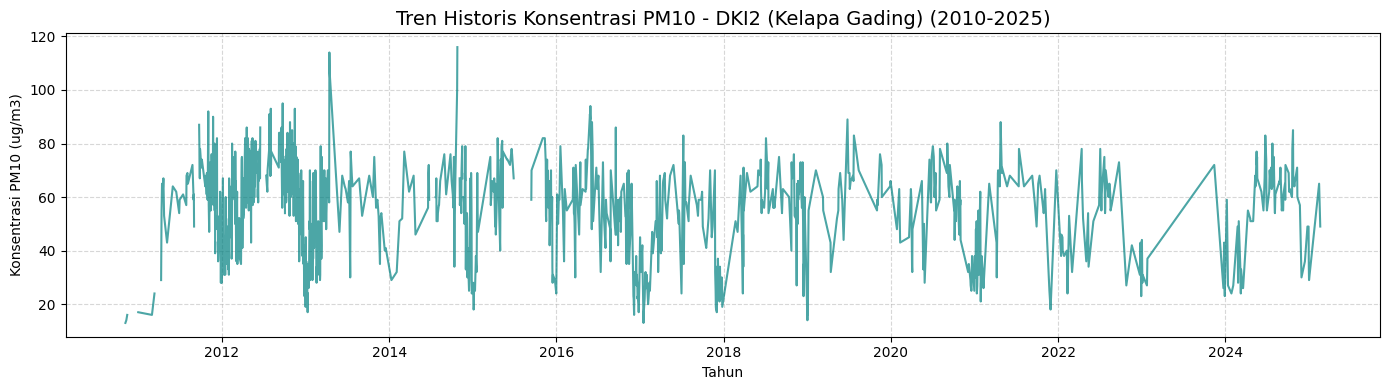
\includegraphics[width=0.8\textwidth]{images/trend_pm10_dki2.png}
  \caption{Tren historis konsentrasi harian PM\textsubscript{10} di Stasiun DKI2 (Kelapa Gading)}
  \label{gambar:trend_dki2}
\end{figure}

\subsubsection{Stasiun DKI3 (Jagakarsa)}

Stasiun DKI3 yang berlokasi di Jakarta Selatan mewakili wilayah dengan tutupan lahan hijau yang relatif lebih luas dibandingkan wilayah administratif lainnya di Jakarta. Karakteristik wilayah ini didominasi oleh permukiman rendah dan area serapan air. Oleh karena itu, profil kualitas udara di Jagakarsa menunjukkan nilai rata-rata konsentrasi polutan yang relatif rendah dalam lingkup pengamatan metropolitan Jakarta. Karakteristik sebaran dan fluktuasi data historis parameter PM\textsubscript{10} pada lokasi ini disajikan secara visual pada Gambar \ref{gambar:trend_dki3}.

\begin{figure}[htbp]
  \centering
  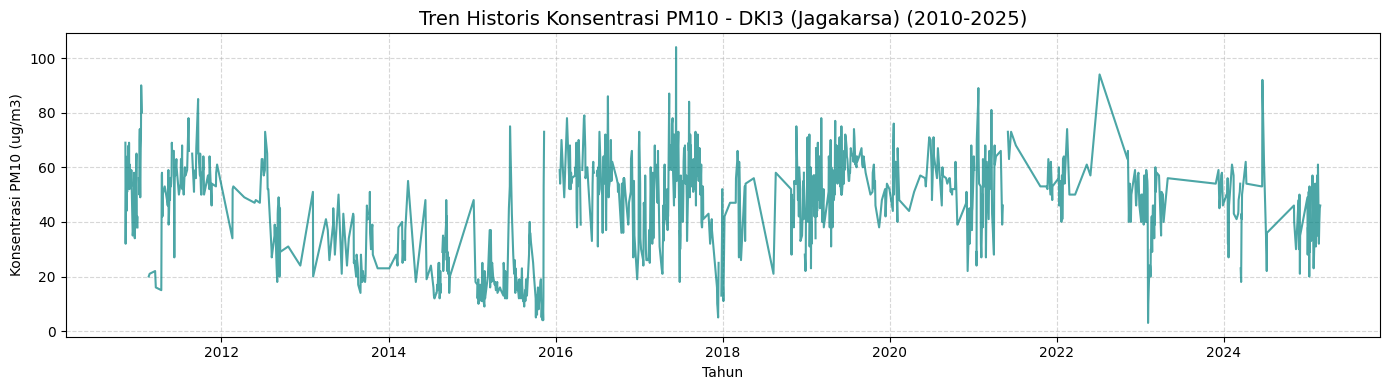
\includegraphics[width=0.8\textwidth]{images/trend_pm10_dki3.png}
  \caption{Tren Historis Konsentrasi Harian PM\textsubscript{10} di Stasiun DKI3 (Jagakarsa)}
  \label{gambar:trend_dki3}
\end{figure}

Visualisasi pada Gambar \ref{gambar:trend_dki3} memperlihatkan bahwa stasiun ini memiliki profil polusi yang moderat dengan nilai puncak yang tidak setinggi kawasan utara atau pusat kota. Meskipun pola fluktuasi musiman tetap teramati mengikuti siklus tahunan, frekuensi lonjakan konsentrasi harian tidak sekerap stasiun pemantau yang berada di kawasan industri atau pusat bisnis. Sifat sebaran data yang cenderung lebih stabil ini menjadikan stasiun DKI3 dapat difungsikan sebagai titik acuan dasar (\textit{baseline}) untuk membandingkan karakteristik pola polusi secara spasial antarwilayah administratif.

Karakteristik data dengan varians yang lebih kecil (\textit{smooth}) di stasiun ini memberikan tantangan tersendiri bagi pemodelan prediktif. Konfigurasi model perlu disesuaikan agar tidak terlalu reaktif terhadap fluktuasi jangka pendek yang kecil guna meminimalkan risiko terjadinya kondisi pembelajaran berlebih (\textit{overfitting}), namun tetap memiliki sensitivitas untuk mendeteksi tren perubahan nilai secara perlahan yang terjadi akibat pertambahan volume aktivitas domestik lokal. Oleh karena itu, fokus pemodelan di stasiun ini diarahkan pada kemampuan algoritma dalam mengenali kecenderungan tren jangka menengah secara konsisten dibandingkan dengan deteksi fluktuasi sesaat.

\subsubsection{Stasiun DKI4 (Lubang Buaya)}

Stasiun DKI4 merepresentasikan karakteristik wilayah permukiman penduduk di sisi Timur Jakarta. Selain aktivitas domestik, wilayah ini juga dipengaruhi oleh pergerakan massa udara dari kawasan industri di daerah penyangga Jakarta. Kombinasi antara karakteristik hunian dan pola angin lokal tersebut memicu penumpukan massa partikulat PM\textsubscript{10} yang tertahan di lapisan atmosfer bawah. Karakteristik sebaran dan fluktuasi data historis polutan pada lokasi ini disajikan secara visual pada Gambar \ref{gambar:trend_dki4}.

\begin{figure}[htbp]
  \centering
  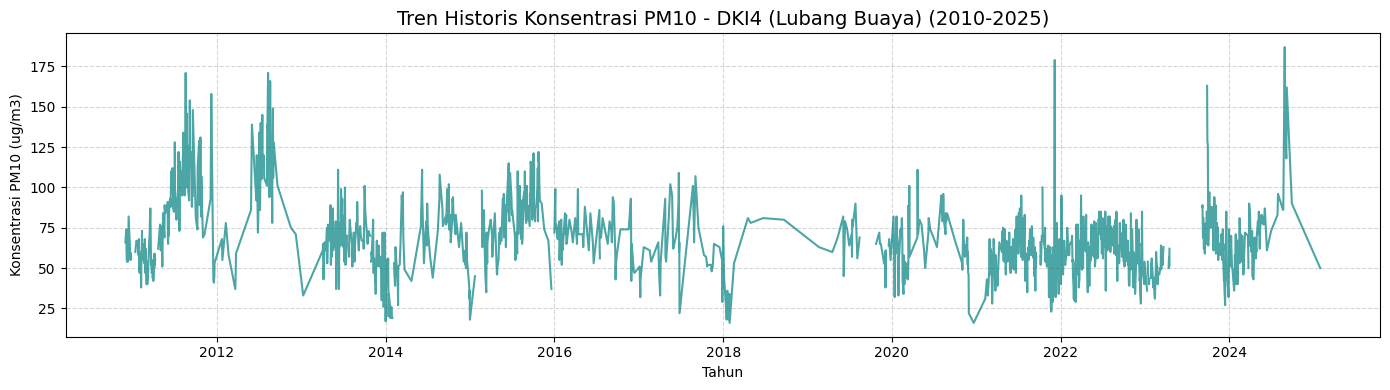
\includegraphics[width=0.8\textwidth]{images/trend_pm10_dki4.png}
  \caption{Tren Historis Konsentrasi Harian PM\textsubscript{10} di Stasiun DKI4 (Lubang Buaya)}
  \label{gambar:trend_dki4}
\end{figure}

Visualisasi pada Gambar \ref{gambar:trend_dki4} memperlihatkan adanya pola persistensi polutan yang tampak jelas di stasiun ini. Nilai konsentrasi berada pada level sedang hingga tinggi dalam rentang waktu tertentu sebelum akhirnya mengalami peluruhan secara bertahap. Fenomena ini mengindikasikan bahwa terdapat ketergantungan temporal pada data historis di lokasi Lubang Buaya, di mana nilai pada hari ini dipengaruhi oleh kondisi beberapa hari sebelumnya.

Karakteristik persistensi tersebut menjadi dasar pertimbangan untuk mengintegrasikan komponen ARIMA dalam arsitektur model hibrida. Kemampuan algoritma statistika dalam menangkap pola autokorelasi linier dinilai sesuai untuk memetakan perilaku polusi di wilayah DKI4. Dengan demikian, kerangka pemodelan hibrida dikonfigurasi untuk memanfaatkan metode statistik konvensional dalam menangkap komponen linier, serta algoritma pembelajaran mesin untuk memetakan pola non-linier lainnya.

\subsubsection{Stasiun DKI5 (Kebon Jeruk)}

Terletak di sisi Barat Jakarta, stasiun DKI5 mencatat dinamika kualitas udara dari kawasan permukiman yang berbatasan dengan koridor transportasi utama antarkota. Lokasi ini dipengaruhi oleh arus lalu lintas harian dari arah daerah penyangga menuju pusat Jakarta, khususnya melalui akses jalan tol. Faktor ini membentuk profil emisi yang bervariasi terhadap volume kendaraan pada jam sibuk komuter harian. Karakteristik sebaran data konsentrasi historis parameter PM\textsubscript{10} pada lokasi ini disajikan secara visual pada Gambar \ref{gambar:trend_dki5}.

\begin{figure}[htbp]
  \centering
  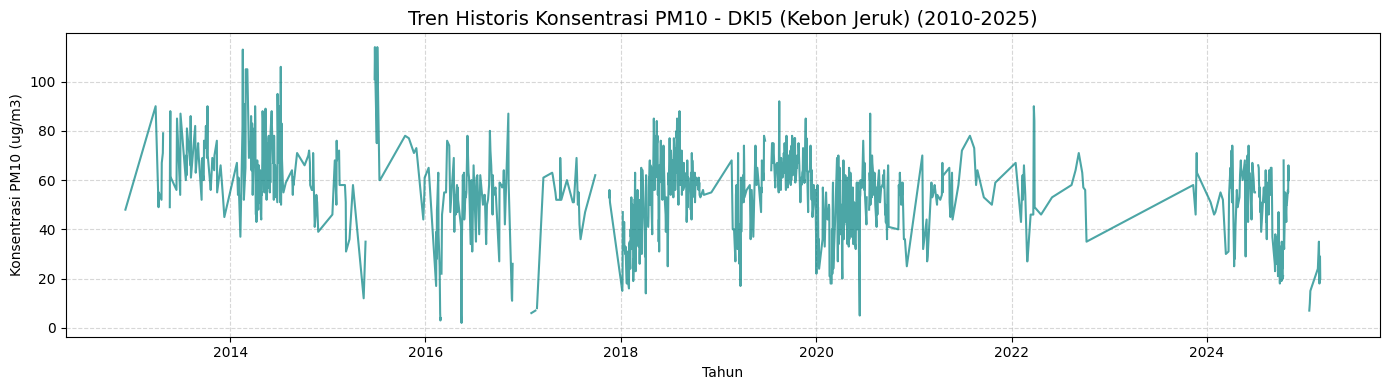
\includegraphics[width=0.8\textwidth]{images/trend_pm10_dki5.png}
  \caption{Tren Historis Konsentrasi Harian PM\textsubscript{10} di Stasiun DKI5 (Kebon Jeruk)}
  \label{gambar:trend_dki5}
\end{figure}

Visualisasi pada Gambar \ref{gambar:trend_dki5} menunjukkan profil PM\textsubscript{10} yang secara umum memiliki kemiripan pola persistensi dengan stasiun DKI4, namun disertai dengan fluktuasi puncak yang tajam. Pola ini mencerminkan adanya akumulasi polutan dari kawasan permukiman sekaligus kontribusi emisi langsung dari kendaraan bermotor yang melintasi koridor utama. Dinamika tersebut menyebabkan data di stasiun DKI5 memiliki struktur berupa gabungan antara komponen linier jangka panjang dan lonjakan non-linier harian.

Sifat data yang bervariasi ini memperkuat pertimbangan dilakukannya analisis secara terpisah per stasiun dalam membangun konfigurasi model prediksi. Meskipun terdapat kemiripan tren umum antar beberapa lokasi, setiap stasiun tetap menyimpan karakteristik tersendiri yang berbeda secara amplitudo dan frekuensi fluktuasi. Oleh karena itu, strategi pelatihan model yang diusulkan diarahkan untuk memastikan setiap stasiun diproses secara mandiri sesuai dengan dinamika lokal masing-masing.

\newpage

\subsection{Analisis Heterogenitas Spasial Melalui Uji Statistik}

Profil data yang telah dipaparkan sebelumnya secara visual menunjukkan adanya perbedaan karakteristik polutan antar stasiun pemantauan. Namun, bukti visual memerlukan validasi uji statistik formal untuk memastikan apakah perbedaan konsentrasi PM\textsubscript{10} antar wilayah administratif Jakarta tersebut terbukti secara statistik atau terjadi karena faktor kebetulan.

Meningat dataset konsentrasi polutan tidak berdistribusi normal (memiliki kemiringan atau \textit{skewness} tertentu), maka digunakan uji statistik non-parametrik Kruskal-Wallis. Uji ini dipilih karena kemampuannya untuk membandingkan lebih dari dua kelompok independen tanpa memerlukan asumsi normalitas data. Hasil dari pengujian ini menjadi penentu apakah model prediksi dapat dibuat secara generalisasi atau harus bersifat spesifik lokasi.

Berdasarkan eksekusi uji Kruskal-Wallis, dihasilkan (\textit{p-value}) yang lebih kecil dari ambang batas 0.05. Temuan ini memberikan justifikasi bahwa distribusi konsentrasi PM\textsubscript{10} pada kelima stasiun pemantauan di DKI Jakarta adalah tidak identik. Konsekuensi dari temuan ini menetapkan bahwa proses pelatihan model tidak dilakukan secara global, lupakan dilatih secara terpisah per stasiun guna menangkap sensitivitas mikroklimat lokal yang spesifik.

\subsection{Analisis Autokorelasi dan Musiman}

Eksplorasi terhadap data deret waktu PM\textsubscript{10} mengonfirmasi adanya ketergantungan temporal melalui analisis \textit{Autocorrelation Function} (ACF) dan \textit{Partial Autocorrelation Function} (PACF). Plot ACF menunjukkan adanya peluruhan eksponensial pada lag-lag awal, yang memberikan bukti empiris mengenai keberadaan sifat otoregresif dalam data. Informasi ini menjadi dasar penggunaan komponen AR dalam kerangka kerja model hibrida RF-ARIMA.

Selain ketergantungan temporal jangka pendek, data polusi di Jakarta juga dipengaruhi oleh faktor meteorologis yang bersifat musiman. Terdapat pola penurunan konsentrasi pada periode Januari hingga Februari akibat proses peluruhan akibat air hujan (\textit{washout effect}) oleh presipitasi curah hujan. Sebaliknya, fenomena inversi termal pada puncak musim kemarau di bulan Juli hingga Agustus menahan partikulat di dekat permukaan tanah, sehingga memengaruhi kenaikan konsentrasi polutan.

Kombinasi antara sifat autokorelasi harian dan tren musiman tahunan ini memerlukan strategi \textit{feature engineering} yang mampu menangkap kedua dimensi tersebut. Penambahan fitur berbasis waktu seperti bulan dan musim, serta fitur \textit{lag} untuk menangkap dependensi temporal, digunakan dalam perancangan model. Dengan demikian, model hibrida yang dikembangkan memiliki kemampuan untuk melakukan estimasi yang adaptif terhadap perubahan kondisi cuaca musiman di Jakarta.

\begin{figure}[htbp]
  \centering
  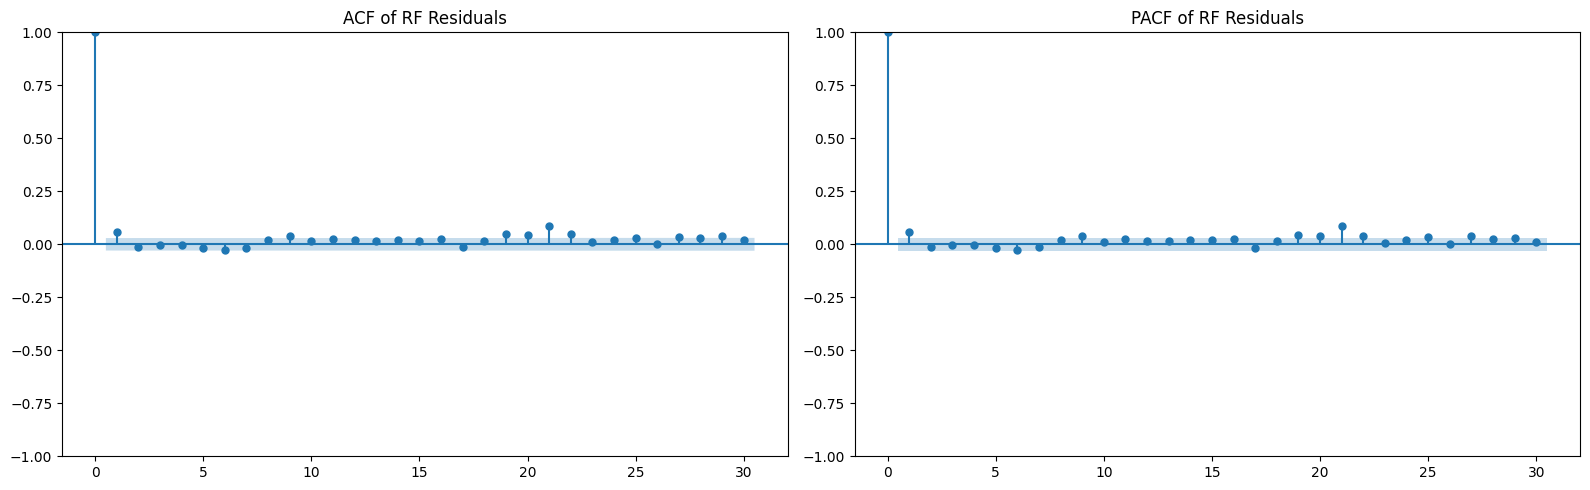
\includegraphics[width=0.8\textwidth]{images/acf_pacf_pm10.png}
  \caption{Plot ACF dan PACF konsentrasi PM\textsubscript{10} Jakarta untuk identifikasi pola autokorelasi temporal}
  \label{gambar:acf_pacf}
\end{figure}

\section{Analisis Domain: Kausalitas dan Dinamika Polutan}

Pemodelan \textit{machine learning} yang tidak mempertimbangkan prinsip fisika atmosferik berisiko menghasilkan regresi spurious atau korelasi semu. Oleh karenanya, dilakukan dekomposisi terhadap mekanisme kausalitas kimiawi dan dinamika temporal antarpolutan sebagai dasar pembentukan arsitektur hibrida dan strategi rekayasa fitur. Analisis domain ini digunakan untuk memastikan bahwa variabel-variabel yang dimasukkan ke dalam model memiliki landasan ilmiah yang sesuai dengan fenomena dispersi dan reaksi kimia udara di wilayah urban.

Integrasi antara pengetahuan domain atmosferik dengan algoritma prediktif bertujuan untuk mempermudah interpretabilitas model. Melalui pemahaman mengenai kontribusi polutan prekursor terhadap pembentukan partikulat, proses ekstraksi fitur tidak lagi dilakukan secara acak, melainkan berbasis pada fenomena fisik. Pendekatan ini dilakukan dalam penelitian ini guna menghubungkan antara akurasi komputasional dengan validitas saintifik.

Hasil analisis pada bagian ini memberikan justifikasi teknis mengenai alasan fitur tertentu, seperti interaksi polutan dan fitur waktu tunda (\textit{lag}), menjadi komponen dalam model hibrida RF-ARIMA. Pemahaman mengenai siklus harian dan musiman polutan di Jakarta digunakan sebagai dasar untuk meminimalkan nilai galat prediksi pada kondisi ekstrem. Penjelasan mengenai korelasi lintas waktu dan mekanisme kimiawi polutan dipaparkan pada sub-bab berikut.

\newpage

\subsection{Analisis Kausalitas Lintas Waktu (\textit{Cross-Correlation Analysis})}

Analisis korelasi silang atau \textit{Cross-Correlation Function} (CCF) dieksekusi untuk menguji adanya ketergantungan temporal antarparameter polutan secara empiris. Analisis ini bertujuan mengukur hubungan antara konsentrasi PM\textsubscript{10} pada waktu $t$ dengan berbagai polutan prekursor pada rentang waktu lampau ($t-k$). Melalui identifikasi jendela waktu tunda di mana pengaruh polutan lain terdeteksi terhadap PM\textsubscript{10}, spesifikasi jendela waktu untuk \textit{lag features} dapat ditentukan. Hasil komputasi dari analisis CCF untuk jendela waktu 7 hari ke belakang divisualisasikan pada Gambar \ref{gambar:ccf_lag}.

\begin{figure}[htbp]
  \centering
  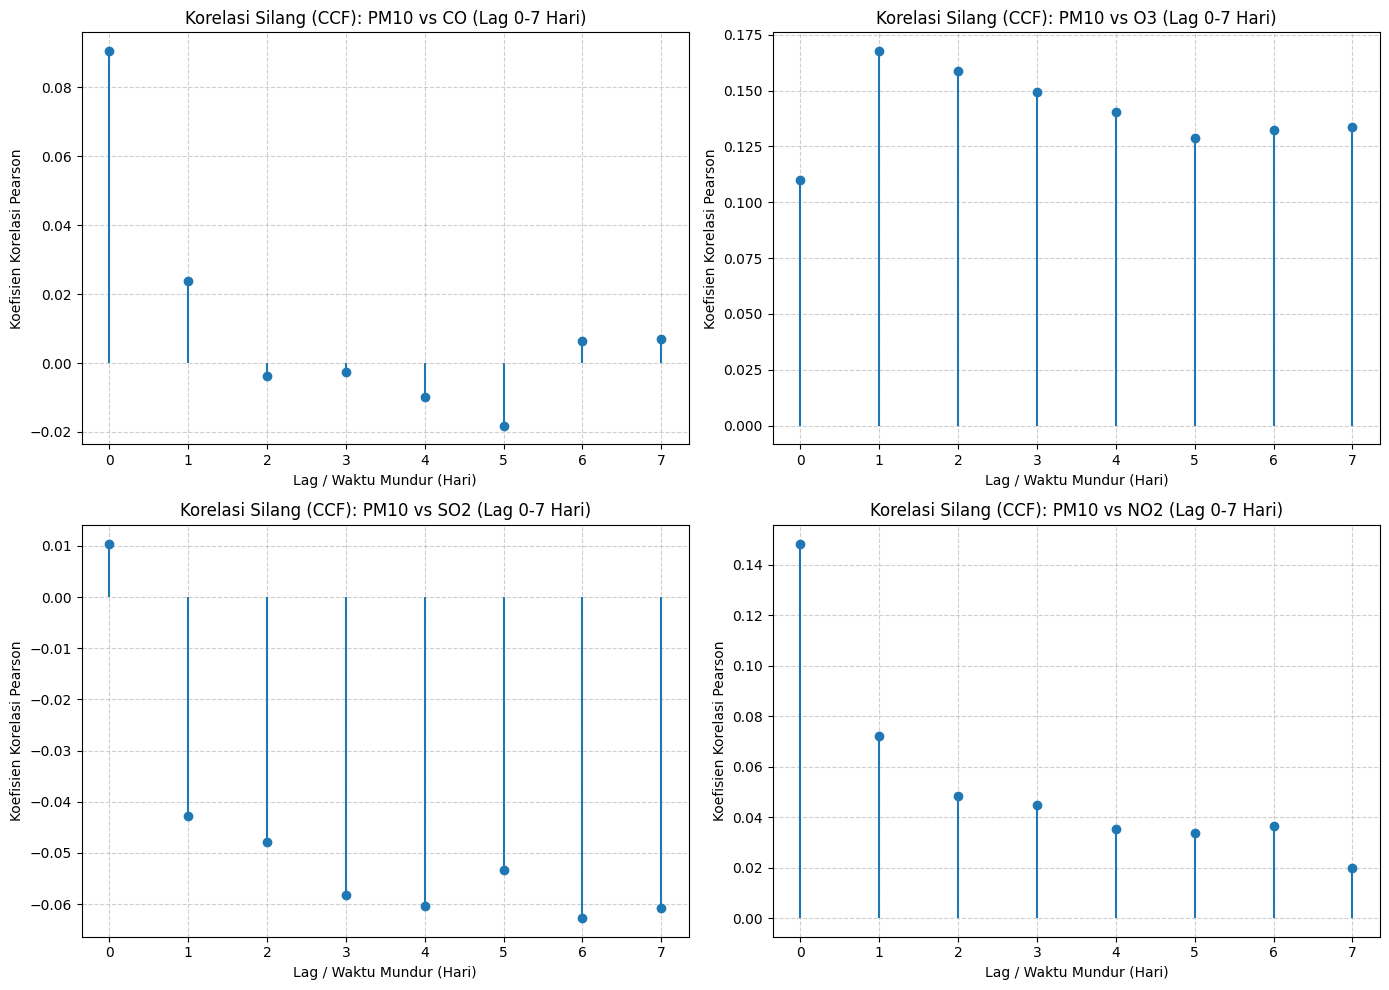
\includegraphics[width=0.8\textwidth]{images/ccf_polutan_lag.png}
  \caption{Analisis Korelasi Silang (CCF) antara PM\textsubscript{10} dengan polutan prekursor pada Lag 0--7 hari}
  \label{gambar:ccf_lag}
\end{figure}

Berdasarkan observasi pada visualisasi di atas, diperoleh temuan utama mengenai persistensi emisi primer seperti Karbon Monoksida (CO) dan Nitrogen Dioksida (NO\textsubscript{2}). Korelasi antara PM\textsubscript{10} dengan kedua polutan tersebut menunjukkan nilai koefisien yang konstan pada Lag 0 ($r > 0,5$), dan terbukti secara statistik hingga rentang Lag 2. Fenomena ini mengindikasikan bahwa emisi kendaraan bermotor yang dilepaskan tidak langsung terdispersi sepenuhnya dari atmosfer Jakarta. Kondisi tersebut dipengaruhi oleh karakteristik lapisan batas planet (\textit{planetary boundary layer}) di wilayah metropolitan yang stabil, sehingga memengaruhi akumulasi massa partikulat dalam rentang waktu beberapa hari.

Selain karakteristik emisi primer, dinamika Ozon Permukaan (O\textsubscript{3}) menunjukkan pola peluruhan korelasi pada rentang Lag 7. Temuan ini mengindikasikan bahwa variasi konsentrasi PM\textsubscript{10} memiliki keterikatan dengan siklus fotokimia mingguan. Perubahan koefisien korelasi yang bertahan pada Lag 1 hingga Lag 3 pada parameter polutan memberikan justifikasi teoretis terhadap penggunaan fitur \textit{lag} dan \textit{rolling window} dalam model. Tanpa menyertakan informasi historis polutan pendukung, estimasi model tidak mengasimilasi konteks akumulasi massa partikulat di atmosfer yang bersifat persisten.

\subsection{Mekanisme Fisik dan Kimia Pembentukan Partikulat Sekunder}

Konsentrasi PM\textsubscript{10} di kawasan perkotaan seperti Jakarta tidak hanya berasal dari emisi primer langsung seperti debu jalan raya dan sisa pembakaran kendaraan, tetapi juga dipengaruhi oleh pembentukan partikulat sekunder hasil reaksi kimia gas di atmosfer yang melibatkan interaksi antar-gas prekursor. Pemahaman terhadap hubungan antar-polutan gas ini menjadi landasan teoretis untuk melakukan tahapan rekayasa fitur, di mana fitur interaksi antar-prediktor digunakan untuk merepresentasikan kecenderungan pembentukan polutan sekunder dalam model. Struktur keterikatan linear secara global untuk seluruh parameter polutan udara independen di wilayah DKI Jakarta melalui perhitungan koefisien korelasi Pearson disajikan secara lengkap pada Gambar \ref{gambar:corr_matrix}.

\begin{figure}[htbp]
  \centering
  \captionsetup{justification=centering}
  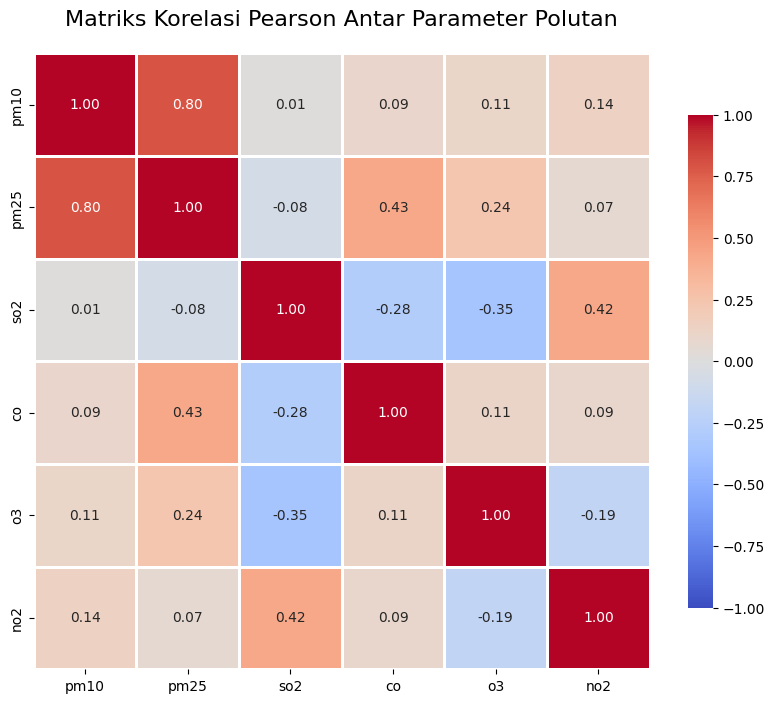
\includegraphics[width=0.6\textwidth]{images/corr_matrix_polutan.png}
  \caption{Matriks Korelasi Pearson Antar Parameter Polutan Udara Jakarta}
  \label{gambar:corr_matrix}
\end{figure}

Berdasarkan matriks korelasi pada Gambar \ref{gambar:corr_matrix}, terlihat adanya pola keterikatan antara gas Karbon Monoksida (CO) dan Ozon Permukaan (O\textsubscript{3}) yang merepresentasikan indikator aktivitas fotokimia di lapisan atmosfer bawah. Selain itu, variasi karakteristik spasial antar-stasiun, seperti wilayah pesisir-logistik DKI2 (Kelapa Gading) yang mencatat fluktuasi gas tertentu akibat aktivitas kendaraan berat, turut memengaruhi sebaran partikulat secara lokal. Pengetahuan domain ini menunjukkan bahwa parameter polutan gas memiliki hubungan interaksi dan efek tunda terhadap konsentrasi PM\textsubscript{10}, sehingga penambahan dimensi fitur komposit diperlukan untuk membantu proses pengenalan pola oleh algoritma hibrida.

\section{Formalisasi Masalah Matematis}

Estimasi nilai konsentrasi polutan PM\textsubscript{10} dalam penelitian ini diformulasikan sebagai sebuah persoalan pemetaan fungsi non-linier yang menggunakan data multivariat historis sebagai variabel masukan. Secara matematis, jika diberikan sebuah deret waktu observasi polutan historis $X = \{x_1, x_2, \dots, x_t\}$, maka tujuan dari model prediktif adalah untuk mengestimasi nilai konsentrasi $y_{t+1}$ pada periode satu hari ke depan. Representasi matematis dari hubungan fungsional antara observasi masa lalu dengan estimasi masa depan tersebut didefinisikan pada Persamaan \ref{eq:formalisasi1}.

\begin{equation}
    y_{t+1} = f(X_t, X_{t-1}, \dots, X_{t-p}) + \epsilon_t
    \label{eq:formalisasi1}
\end{equation}
\eqcaption{Formulasi Pemetaan Fungsi Prediksi Deret Waktu Multivariat}

Dalam perumusan tersebut, variabel $f(\cdot)$ merepresentasikan fungsi transformasi regresi yang bersifat agregat, sementara $p$ menunjukkan ordo jendela waktu lampau atau jeda temporal yang digunakan untuk menangkap karakteristik dependensi temporal dari data deret waktu. Komponen $\epsilon_t$ didefinisikan sebagai sisaan acak yang tidak dapat dipetakan secara deterministik oleh model. 

Pendekatan ini didasarkan pada asumsi bahwa data kualitas udara mengandung pola-pola yang dapat diurai berdasarkan karakteristik statistiknya melalui teorema dekomposisi. Berdasarkan prinsip tersebut, fungsi pemetaan $y_t$ dibagi menjadi dua komponen terpisah sebagaimana dinyatakan pada Persamaan \ref{eq:formalisasi2}.

\begin{equation}
    y_t = L_t + N_t
    \label{eq:formalisasi2}
\end{equation}
\eqcaption{Dekomposisi Sinyal Polutan Menjadi Komponen Linier dan Non-Linier}

Komponen $L_t$ pada Persamaan \ref{eq:formalisasi2} merepresentasikan fungsi linier yang memiliki sifat autokorelasi, di mana komponen ini dimodelkan menggunakan persamaan diferensi stokastik ARIMA. Sementara itu, komponen $N_t$ mewakili fungsi non-linier—seperti pengaruh interaksi antarpolutan dan variasi meteorologi—yang dipetakan secara non-parametrik melalui struktur ensambel pohon keputusan \textit{Random Forest}. 

Penggabungan kedua komponen ini secara hibrida ditujukan untuk meminimalkan keterbatasan model regresi tunggal yang memiliki batasan dalam memproses karakteristik data yang bervariasi, sehingga diharapkan dapat mengurangi nilai galat estimasi terhadap dinamika atmosfer Jakarta yang fluktuatif.

\section{Desain Ekstraksi Fitur Deret Waktu (\textit{Feature Engineering})}

Berdasarkan hasil analisis karakteristik data spasial dan kausalitas domain atmosferik pada subbab sebelumnya, rancangan spesifikasi fitur disusun secara sistematis. Proses rekayasa fitur (\textit{feature engineering}) ini berfungsi untuk mengekstraksi informasi prediktif yang terdapat di dalam deret waktu mentah agar dapat diproses oleh model komputasi. Tanpa adanya transformasi fitur yang memadai, model \textit{machine learning} memiliki keterbatasan dalam memetakan pola karakteristik pada data lingkungan yang memiliki derau (\textit{noise}).

Dalam penelitian ini, dirancang spesifikasi ekstraksi untuk menghasilkan 15 fitur komputasional yang dimasukkan ke dalam arsitektur model hibrida. Ekstraksi fitur ini bertujuan untuk menyediakan representasi variabel yang bervariasi secara multivariat. Komponen yang diekstrak mencakup aspek dependensi temporal, distribusi statistik lokal, interaksi kimiawi antarpolutan, serta pola waktu deterministik yang berulang secara periodik.

Secara matematis, proses rekayasa fitur ini dideskripsikan ke dalam empat kategori utama. Setiap kategori memiliki fungsi dalam memetakan fenomena fisik atmosfer ke dalam variabel numerik yang dapat dikomputasi. Deskripsi, justifikasi fisis, dan formulasi matematis dari masing-masing kategori fitur diuraikan pada sub-bagian berikut.

\subsection{Fitur Jeda Temporal (\textit{Lag Features})}

Ekstraksi fitur jeda temporal atau \textit{lag features} digunakan untuk menangkap efek persistensi dari polutan di atmosfer. Di wilayah urban seperti DKI Jakarta, laju disipasi emisi kendaraan bermotor maupun debu jalanan membutuhkan waktu untuk terurai atau terdispersi oleh angin. Kondisi ini menyebabkan konsentrasi PM\textsubscript{10} pada rentang waktu saat ini dipengaruhi oleh akumulasi massa partikulat dari hari-hari sebelumnya.

Berdasarkan analisis fungsi autokorelasi (ACF) yang dieksekusi pada tahap \textit{data profiling}, rentang batas jeda waktu ditentukan hingga tujuh hari ke belakang ($t-7$). Rentang waktu ini dinilai merepresentasikan peluruhan dari polutan primer sebelum akhirnya kehilangan nilai keterikatan statistik. Penggunaan fitur jeda yang terlalu panjang memerlukan pertimbangan agar tidak menambah nilai kesalahan (\textit{noise}) yang dapat memengaruhi hasil estimasi prediksi.

Proses ekstraksi ini memetakan nilai historis masa lalu menjadi fitur prediktor independen pada matriks pelatihan. Fitur yang diekstraksi meliputi konsentrasi polutan pada satu hari sebelumnya (PM10\textsubscript{t-1}) hingga tujuh hari sebelumnya (PM10\textsubscript{t-7}). Formulasi matematis dari pembentukan \textit{lag features} ditunjukkan pada Persamaan \ref{eq:lag_features}.

\begin{equation}
    L_k = X_{t-k}, \quad \text{untuk } k \in \{1, 2, \dots, 7\}
    \label{eq:lag_features}
\end{equation}
\eqcaption{Formulasi Ekstraksi Fitur Jeda Temporal}

\subsection{Fitur Statistik Jendela Berjalan (\textit{Rolling Window Statistics})}

Kondisi kualitas udara di Jakarta dipengaruhi oleh siklus aktivitas harian masyarakat yang berulang setiap minggunya. Untuk merepresentasikan pola pergerakan tersebut, digunakan teknik ekstraksi fitur berbasis jendela observasi berjalan (\textit{rolling window}) dengan rentang waktu 3-hari ($W=3$) dan 7-hari ($W=7$) untuk menghitung metrik statistik lokal yang merangkum dinamika polusi jangka pendek dan mingguan.

Metrik pertama yang diekstraksi adalah rata-rata bergerak (\textit{Rolling Mean}) 3-hari (\texttt{pm10\_ma3}) dan 7-hari (\texttt{pm10\_ma7}), yang berfungsi untuk menghaluskan fluktuasi harian dan memberikan nilai dasar polusi berkala. Metrik kedua adalah standar deviasi berjalan (\textit{Rolling Standard Deviation}) 7-hari (\texttt{pm10\_std7}), yang bertindak sebagai proksi matematis untuk mendeteksi derajat volatilitas data atau adanya perubahan cuaca harian dalam periode satu minggu tersebut.

Kombinasi dari metrik statistik ini memungkinkan model \textit{Random Forest} untuk memahami apakah data observasi harian berada dalam kondisi normal, sedang mengalami tren perubahan nilai, atau merupakan fluktuasi sesaat. Kalkulasi matematis untuk masing-masing fitur statistik jendela berjalan diturunkan pada Persamaan \ref{eq:roll_mean3}, Persamaan \ref{eq:roll_mean7}, dan Persamaan \ref{eq:roll_std7}.

\begin{equation}
    RM_{3} = \frac{1}{3} \sum_{i=1}^{3} \text{PM10}_{t-i}
    \label{eq:roll_mean3}
\end{equation}
\eqcaption{Formulasi Rata-rata Jendela Berjalan 3 Hari}

\begin{equation}
    RM_{7} = \frac{1}{7} \sum_{i=1}^{7} \text{PM10}_{t-i}
    \label{eq:roll_mean7}
\end{equation}
\eqcaption{Formulasi Rata-rata Jendela Berjalan 7 Hari}

\begin{equation}
    RStd_{7} = \sqrt{\frac{1}{6} \sum_{i=1}^{7} (\text{PM10}_{t-i} - RM_{7})^2}
    \label{eq:roll_std7}
\end{equation}
\eqcaption{Formulasi Standar Deviasi Jendela Berjalan 7 Hari}

\subsection{Fitur Interaksi Polutan dan Karakteristik Oksidasi}

Berdasarkan analisis domain atmosfer, pembentukan partikulat sekunder dikatalisasi oleh keberadaan polutan pendukung lainnya. Algoritma \textit{machine learning} konvensional mengasumsikan setiap fitur input bersifat independen, sehingga interaksi antarvariabel secara statistik kerap tidak tertangkap secara langsung. Oleh karenanya, model ditambahkan fitur interaksi perkalian guna merepresentasikan laju reaksi polutan tersebut.

Fitur interaksi dibangun dengan menghitung hasil kali konsentrasi Karbon Monoksida (CO) dan Ozon Permukaan (O\textsubscript{3}) untuk memodelkan indikator oksidasi fotokimia (\texttt{co\_times\_o3}). Karbon Monoksida bertindak sebagai indikator emisi primer kendaraan, sedangkan Ozon merupakan penanda derajat transisi cuaca panas. 

Melalui penyusunan fitur interaksi perkalian ini, model \textit{Random Forest} dapat mengidentifikasi kondisi pembentukan polutan sekunder secara lebih efisien tanpa memerlukan kedalaman percabangan pohon keputusan yang tinggi. Formulasi matematis dari fitur interaksi dideskripsikan pada Persamaan \ref{eq:int_co}.

\begin{equation}
    Int(CO, O_3) = CO_t \times O_{3,t}
    \label{eq:int_co}
\end{equation}
\eqcaption{Formulasi Fitur Interaksi Karbon Monoksida dan Ozon}

\subsection{Fitur Temporal dan Siklus Aktivitas}

Komponen waktu seperti tanggal tidak diproses secara langsung oleh algoritma regresi karena sifatnya yang berupa deret numerik kontinu. Oleh sebab itu, komponen waktu ditransformasi menjadi dimensi spasial diskrit guna menangkap tren perulangan aktivitas masyarakat dan variasi musiman harian. Ekstraksi fitur waktu ini digunakan untuk menyediakan informasi penanggalan kepada model.

\newpage

Fitur pertama yang dibentuk adalah indeks hari dalam satu minggu (\textit{Day of Week}), yang dikalkulasi menggunakan operasi modulo pada indeks hari berurutan. Transformasi ini bertujuan agar model memetakan urutan hari kerja yang menunjukkan karakteristik volume kendaraan yang stabil. Selain itu, fitur kategorikal biner \texttt{is\_weekend} juga ditambahkan untuk menandai hari Sabtu dan Minggu secara eksklusif. 

Penggunaan fitur biner \texttt{is\_weekend} dirancang untuk merepresentasikan penurunan nilai fluktuasi volume kendaraan komuter lintas daerah ke pusat perkotaan, yang memengaruhi penurunan pola polutan di akhir pekan. Representasi matematis untuk transformasi indeks hari menjadi ruang vektor diskrit ditunjukkan pada Persamaan \ref{eq:dayofweek}.

\begin{equation}
    \text{DayOfWeek}_t = t \pmod 7
    \label{eq:dayofweek}
\end{equation}
\eqcaption{Formulasi Transformasi Siklus Hari dalam Seminggu}

\section{Analisis Kebutuhan Sistem}

Analisis kebutuhan sistem merupakan tahapan penting dalam siklus pengembangan sistem prediktif yang bertujuan untuk mendefinisikan batasan, kapabilitas, dan ekspektasi performa dari artefak yang akan dibangun. Proses ini dilakukan untuk memastikan bahwa solusi teknis yang diusulkan, yakni model hibrida RF-ARIMA, selaras dengan urgensi pemecahan masalah polusi udara di DKI Jakarta. Melalui identifikasi kebutuhan secara mendalam, seluruh fungsi sistem dapat dirancang secara terukur untuk meminimalkan kendala latensi informasi dan keterbatasan transparansi model yang telah diidentifikasi pada tahapan sebelumnya.

\subsection{Identifikasi Masalah Pengguna dan Pemetaan Regulasi}

Perancangan model prediktif ini diselaraskan dengan kepatuhan terhadap standar regulasi nasional yang berlaku di Indonesia, khususnya Peraturan Menteri Lingkungan Hidup dan Kehutanan (Permen LHK) Nomor 14 Tahun 2020 tentang Indeks Standar Pencemar Udara. Regulasi tersebut menjadi acuan dasar dalam menentukan parameter polutan harian dan ambang batas konsentrasi guna menjaga keselarasan hukum serta teknis teknis dari luaran model. Selain aspek regulasi, kebutuhan fungsional dari otoritas pengambil kebijakan terkait juga menjadi faktor pendorong di mana instansi memerlukan alat bantu yang memproses data historis sekaligus memberikan estimasi kondisi kualitas udara untuk periode mendatang. Ketersediaan informasi penaksiran nilai ini didesain agar pihak berwenang dapat mempertimbangkan langkah preventif, seperti pengelolaan mobilitas kendaraan atau penyampaian panduan kesehatan, sebelum konsentrasi polutan berada pada tingkat yang dapat memengaruhi kesehatan masyarakat.

Sintesis antara analisis masalah pengguna dan pemetaan regulasi tersebut menghasilkan tiga kategori kebutuhan operasional yang mendasari pengembangan konfigurasi model hibrida ini. Kategori pertama adalah kebutuhan estimasi harian yang proaktif sebagai fungsi informasi dini terhadap fluktuasi polutan harian untuk horizon waktu satu hari ke depan ($t+1$). Kategori kedua berfokus pada aspek transparansi model, di mana kerangka kerja menyediakan kejelasan mengenai distribusi kontribusi fitur masukan untuk membantu proses penelaahan dasar keputusan model secara objektif. Kategori terakhir adalah fleksibilitas spasial yang memerlukan penyesuaian parameter model agar adaptif terhadap karakteristik mikroklimat yang bervariasi pada masing-masing stasiun pemantauan di wilayah DKI Jakarta.

\subsection{Kebutuhan Fungsional}

Kebutuhan fungsional menetapkan kapabilitas teknis dan operasional yang harus dimiliki oleh sistem untuk mencapai tujuan estimasi konsentrasi polutan PM\textsubscript{10}. Fokus utama dari parameter fungsional ini meliputi pengelolaan alur data secara terintegrasi, mulai dari tahap penarikan berkas data historis hingga penaksiran nilai melalui modul komputasi hibrida sekuensial. Modul pemrosesan dirancang untuk mengeksekusi rangkaian logika transformasi prediktor secara bertahap guna menghasilkan nilai luaran berupa proyeksi tingkat polusi untuk satu hari ke depan ($t+1$). Rincian mengenai deskripsi kebutuhan fungsional sistem ini dijabarkan secara sistematis pada Tabel \ref{tbl:fungsional}.

Selain aspek pemodelan utama, sistem memfasilitasi fungsionalitas pendukung untuk penjaminan kualitas data (\textit{data quality assurance}). Aturan fungsional ini mencakup proses pembersihan data dari nilai ekstrem serta penanganan terhadap data hilang (\textit{missing values}) yang kerap terjadi pada perangkat sensor pemantau di lapangan. Integrasi modul rekayasa fitur juga menjadi bagian inti agar fungsi komputasi dapat mengekstrak variabel jeda temporal dan interaksi kimiawi antarpolutan yang telah dirancang sebelumnya.

Aspek lain dari kebutuhan fungsional adalah penyediaan mekanisme evaluasi dan interpretasi model secara otomatis setelah proses pelatihan selesai. Modul prediktif tidak hanya mengeluarkan nilai taksiran numerik, tetapi juga menghitung metrik kesalahan statistik untuk memvalidasi performa hasil peramalan secara periodik. Lebih lanjut, keberadaan modul \textit{Explainable Artificial Intelligence} (XAI) menjadi fungsi pelengkap untuk menguraikan kontribusi dan pengaruh dari masing-masing fitur masukan terhadap pembentukan nilai prediksi akhir.

\begin{table}[htbp]
\centering
\captionsetup{justification=centering}
\setlength{\tabcolsep}{6pt} 
\caption{Kebutuhan Fungsional Sistem Pemodelan PM\textsubscript{10}}
\label{tbl:fungsional}

\begin{tabularx}{\textwidth}{|>{\centering\arraybackslash}p{1.0cm}|
                              >{\centering\arraybackslash}p{1.8cm}|
                              >{\raggedright\arraybackslash}X|}
\hline
\textbf{No.} & \textbf{Kode} & \textbf{Deskripsi Kebutuhan Fungsional}\\
\hline
1 & F-01 & Memprediksi nilai konsentrasi harian $PM_{10}$ di wilayah DKI Jakarta menggunakan basis data deret waktu historis. \\
\hline
2 & F-02 & Mengeksekusi peramalan melalui implementasi arsitektur hibrida sekuensial menggabungkan \textit{Random Forest} (RF) dan ARIMA. \\
\hline
3 & F-03 & Mentransformasi data mentah menjadi 15 fitur komputasional melalui tahapan rekayasa fitur (\textit{feature engineering}). \\
\hline
4 & F-04 & Menghitung metrik evaluasi performa regresi secara otomatis, meliputi nilai RMSE, MAE, dan Koefisien Determinasi ($R^2$). \\
\hline
5 & F-05 & Mengintegrasikan modul \textit{Explainable AI} (XAI) untuk menghitung dan memvisualisasikan kontribusi fitur menggunakan nilai SHAP. \\
\hline
6 & F-06 & Memfasilitasi fungsi pembersihan data (\textit{data cleaning}) untuk dataset kualitas udara berformat tabular periode 2010--2025. \\
\hline
\end{tabularx}
\end{table}

\subsection{Kebutuhan Nonfungsional}

Kebutuhan nonfungsional menetapkan batasan operasional dan atribut kualitas yang menentukan derajat keandalan sistem saat seluruh modul dieksekusi. Atribut kualitas ini tidak berkaitan dengan penyediaan fitur spesifik, melainkan pada bagaimana seluruh elemen komputasi berperilaku di bawah batasan teknis lingkungan peladen harian. Fokus utama pada bagian ini meliputi performa batas nilai galat, ketangguhan konfigurasi model terhadap variansi data, serta efisiensi penggunaan alokasi memori perangkat keras saat menjalankan proses inferensi hibrida. Rincian deskripsi mengenai kebutuhan nonfungsional sistem disajikan pada Tabel \ref{tbl:nonfungsional}.

Salah satu parameter kualitas operasional yang ditargetkan adalah aspek akurasi relatif dan stabilitas estimasi model. Arsitektur hibrida sekuensial yang dikembangkan dikondisikan untuk menunjukkan nilai kesalahan (galat) penaksiran yang lebih rendah jika dibandingkan dengan performa model tunggal murni yang diposisikan sebagai acuan dasar (\textit{baseline}). Selain itu, model menggunakan mekanisme validasi temporal guna meminimalkan risiko algoritma mengalami kondisi penyesuaian berlebih (\textit{overfitting}) terhadap parameter data latih.

\newpage

Aspek keterulangan (\textit{reproducibility}) dan transparansi operasional juga menjadi karakteristik kualitas penting dalam perancangan tugas akhir ini. Seluruh siklus komputasi dirancang sedemikian rupa agar alur pemrosesan dari tahap prapemrosesan data hingga visualisasi taksiran akhir dapat direplikasi pada lingkungan eksekusi yang berbeda tanpa mengubah hasil luaran numerik. Hal ini dilakukan agar keandalan model hibrida yang dihasilkan dapat diuji validitas keilmuannya secara terbuka dan konsisten pada ekosistem pemrograman Python.

\begin{table}[htbp]
\centering
\captionsetup{justification=centering}
\setlength{\tabcolsep}{6pt} 
\caption{Kebutuhan Nonfungsional Sistem Pemodelan PM\textsubscript{10}}
\label{tbl:nonfungsional}

\begin{tabularx}{\textwidth}{|>{\centering\arraybackslash}p{1.0cm}|
                              >{\centering\arraybackslash}p{1.8cm}|
                              >{\raggedright\arraybackslash}X|}
\hline
\textbf{No.} & \textbf{Kode} & \textbf{Deskripsi Kebutuhan Nonfungsional}\\
\hline
1 & NF-01 & {Akurasi Relatif:} Menghasilkan nilai galat (RMSE) model hibrida yang lebih rendah dibandingkan model tunggal murni (\textit{baseline}). \\
\hline
2 & NF-02 & {Robustness:} Meminimalkan risiko \textit{overfitting} melalui implementasi \textit{Time-Series Cross-Validation} berbasis \textit{TimeSeriesSplit} 5-\textit{fold}. \\
\hline
3 & NF-03 & {Interpretabilitas:} Mengeksekusi nilai atribusi fitur algoritma SHAP dalam batas memori peladen harian tanpa memicu kegagalan sistem. \\
\hline
4 & NF-04 & {Reproduksibilitas:} Menjamin seluruh siklus komputasi dari prapemrosesan hingga estimasi dapat direplikasi secara konsisten di lingkungan Python. \\
\hline
\end{tabularx}
\end{table}

\section{Analisis Pemilihan Paradigma Melalui \textit{Analytical Hierarchy Process}}

Pemilihan arsitektur pemodelan untuk estimasi kualitas udara memerlukan pertimbangan komprehensif yang tidak hanya mencakup aspek akurasi statistik, melainkan juga batasan operasional administratif instansi terkait. Metode \textit{Analytical Hierarchy Process} (AHP) diterapkan pada tahapan ini sebagai kerangka kerja pengambilan keputusan terstruktur untuk mengevaluasi dan membandingkan beberapa alternatif solusi arsitektur pemodelan secara objektif. Melalui pendekatan hierarki ini, berbagai kriteria teknis maupun non-teknis disintesis secara sistematis guna menentukan paradigma solusi awal yang paling sesuai untuk diimplementasikan pada infrastruktur sistem informasi pemantauan lingkungan di DKI Jakarta.

\subsection{Justifikasi Penggunaan AHP Sebelum Evaluasi Empiris}

Sebuah catatan metodologis perlu dikemukakan terkait penggunaan \textit{Analytical Hierarchy Process} (AHP) dalam penelitian tugas akhir berbasis sains data ini. Pada umumnya, pemilihan arsitektur model prediksi ditentukan murni secara empiris berdasarkan metrik kinerja kuantitatif (seperti nilai RMSE) setelah seluruh rangkaian eksperimen selesai dijalankan. Namun, dalam konteks implementasi sistem informasi pada instansi pemerintahan lokal seperti Dinas Lingkungan Hidup DKI Jakarta, batasan operasional tidak hanya bergantung pada dimensi akurasi statistik semata. Terdapat parameter multi-kriteria non-teknis administratif yang harus dipenuhi, seperti tingkat transparansi keputusan (interpretabilitas) agar hasil prakiraan dapat ditelaah secara logis, efisiensi alokasi infrastruktur peladen harian, serta kemudahan replikasi kode operasional sistem.

Oleh karena itu, kerangka kerja AHP pada penelitian ini tidak diposisikan sebagai pengganti evaluasi kinerja empiris model akhir, melainkan sebagai instrumen analisis kebutuhan pra-eksperimen (\textit{pre-development framework}) untuk menjustifikasi pemilihan paradigma arsitektur awal. Tahap evaluasi awal ini dilakukan dengan menyusun matriks perbandingan berpasangan (\textit{pairwise comparison}) untuk lima kriteria operasional, yaitu Interpretabilitas (INT), Akurasi (AKR), Kemampuan Menangkap Pola Kompleks (PLK), Efisiensi Komputasi (KMP), dan Kemudahan Implementasi (IMP). 

Dalam konteks penyediaan informasi kualitas udara harian, kriteria INT, AKR, dan PLK diberikan bobot kepentingan yang lebih tinggi, sedangkan kriteria KMP dan IMP diberikan bobot yang lebih rendah karena aktivitas peramalan diproses secara berkala (\textit{batch processing}). Nilai kepentingan relatif antar-kriteria tersebut disajikan pada Tabel \ref{tbl:pairwise_kriteria}.

\begin{table}[htbp]
\centering
\captionsetup{justification=centering}
\setlength{\tabcolsep}{4pt} 
\caption{Matriks Perbandingan Berpasangan Kriteria Utama}
\label{tbl:pairwise_kriteria}

\begin{tabularx}{\textwidth}{|>{\raggedright\arraybackslash}X|
                              >{\centering\arraybackslash}p{1.3cm}|
                              >{\centering\arraybackslash}p{1.3cm}|
                              >{\centering\arraybackslash}p{1.3cm}|
                              >{\centering\arraybackslash}p{1.3cm}|
                              >{\centering\arraybackslash}p{1.3cm}|}
\hline
\textbf{Kriteria} & \textbf{INT} & \textbf{AKR} & \textbf{PLK} & \textbf{KMP} & \textbf{IMP} \\
\hline
Interpretabilitas (INT) & 1,00 & 1,20 & 2,50 & 3,00 & 4,00 \\
\hline
Akurasi (AKR) & 0,83 & 1,00 & 2,00 & 3,00 & 3,00 \\
\hline
Pola Kompleks (PLK) & 0,40 & 0,50 & 1,00 & 2,00 & 2,00 \\
\hline
Komputasi (KMP) & 0,33 & 0,33 & 0,50 & 1,00 & 1,00 \\
\hline
Implementasi (IMP) & 0,25 & 0,33 & 0,50 & 1,00 & 1,00 \\
\hline
\textbf{Jumlah} & \textbf{2,81} & \textbf{3,36} & \textbf{6,50} & \textbf{10,00} & \textbf{11,00} \\
\hline
\end{tabularx}
\end{table}

Kalkulasi dilanjutkan dengan melakukan proses normalisasi matriks melalui pembagian setiap elemen baris dengan jumlah total nilai pada kolom bersesuaian. Vektor bobot prioritas global (\textit{Eigenvector}) kemudian diperoleh melalui perhitungan nilai rata-rata baris dari matriks yang telah dinormalisasi. Nilai bobot prioritas global ini berfungsi sebagai parameter pengali untuk menentukan solusi paradigma arsitektur pemodelan yang dinilai memenuhi keselarasan kebutuhan administratif instansi, sebagaimana hasil perhitungan yang dirangkum pada Tabel \ref{tbl:eigen_kriteria}.

\newpage

\begin{table}[htbp]
\centering
\captionsetup{justification=centering}
\setlength{\tabcolsep}{4pt} 
\caption{Matriks Normalisasi dan Perhitungan \textit{Eigenvector} Kriteria}
\label{tbl:eigen_kriteria}

\begin{tabularx}{\textwidth}{|>{\raggedright\arraybackslash}X|
                              >{\centering\arraybackslash}p{1.2cm}|
                              >{\centering\arraybackslash}p{1.2cm}|
                              >{\centering\arraybackslash}p{1.2cm}|
                              >{\centering\arraybackslash}p{1.2cm}|
                              >{\centering\arraybackslash}p{1.2cm}|
                              >{\centering\arraybackslash}p{2.2cm}|}
\hline
\textbf{Kriteria} & \textbf{INT} & \textbf{AKR} & \textbf{PLK} & \textbf{KMP} & \textbf{IMP} & \textbf{Prioritas (\textit{W})} \\
\hline
INT & 0,356 & 0,357 & 0,385 & 0,300 & 0,364 & \textbf{0,352} \\
\hline
AKR & 0,295 & 0,298 & 0,308 & 0,300 & 0,273 & \textbf{0,295} \\
\hline
PLK & 0,142 & 0,149 & 0,154 & 0,200 & 0,182 & \textbf{0,165} \\
\hline
KMP & 0,117 & 0,098 & 0,077 & 0,100 & 0,091 & \textbf{0,097} \\
\hline
IMP & 0,089 & 0,098 & 0,077 & 0,100 & 0,091 & \textbf{0,091} \\
\hline
\end{tabularx}
\end{table}

\subsection{Uji Konsistensi Matriks}

Untuk menjamin bahwa penilaian hierarki beserta pembobotan bersifat logis secara matematis, dilakukan uji konsistensi matriks. Proses ini digunakan untuk meminimalkan risiko terjadinya rasio penilaian yang saling bertentangan. Langkah awal dalam pengujian ini adalah mengkalkulasi Nilai Eigen Maksimum ($\lambda_{max}$) yang direpresentasikan melalui persamaan dot produk antara jumlah metrik kolom dengan vektor bobot prioritas sebagai berikut:

\begin{equation}
    \lambda_{max} = (2,81 \times 0,352) + (3,36 \times 0,295) + \dots + (11,00 \times 0,091) = 5,165
    \label{eq:lambda_max}
\end{equation}

Setelah diperoleh nilai eigen maksimum, langkah selanjutnya adalah menghitung \textit{Consistency Index} (CI). Indeks ini mengukur seberapa jauh matriks evaluasi menyimpang dari kondisi konsisten, dengan mempertimbangkan jumlah dimensi kriteria ($n=5$), yang diformulasikan melalui Persamaan \ref{eq:ci}.

\begin{equation}
    CI = \frac{\lambda_{max} - n}{n - 1} = \frac{5,165 - 5}{4} = 0,041
    \label{eq:ci}
\end{equation}

Langkah penutup dari validasi ini adalah komputasi batas penerimaan melalui formula \textit{Consistency Ratio} (CR). Rasio ini membandingkan nilai CI terhadap sebuah indeks acak standar (\textit{Random Index} atau $RI$) yang bernilai 1,12 untuk matriks berukuran $5 \times 5$, sebagaimana ditunjukkan pada Persamaan \ref{eq:cr}.

\begin{equation}
    CR = \frac{CI}{RI} = \frac{0,041}{1,12} = 0,037
    \label{eq:cr}
\end{equation}

Berdasarkan hasil pembagian pada Persamaan \ref{eq:cr}, diperoleh nilai batas sebesar 0,037 yang berada di bawah toleransi ketidaksesuaian maksimum sebesar 0,1. Dengan demikian, kerangka kriteria AHP dinyatakan valid untuk digunakan dalam menentukan bobot prioritas.

\subsection{Penilaian Alternatif Berdasarkan Kriteria}

Tahap evaluasi alternatif menguji secara komparatif kemampuan komputasional dari setiap arsitektur solusi terhadap masing-masing kriteria yang telah ditentukan batasan nilainya. Proses ini dilaksanakan dengan membentuk matriks perbandingan berpasangan lokal berskala 3x3 untuk menilai ketiga kandidat (ARIMA, \textit{Random Forest}, dan Hibrida) secara terpisah. Tujuannya adalah untuk menganalisis karakteristik dari setiap algoritma secara mandiri.

Prosedur ini mengacu pada metodologi dekomposisi, di mana batasan dari satu arsitektur akan tercermin pada nilai prioritas lokal yang bersangkutan. Hal ini dilakukan agar analisis didasarkan pada pengukuran kriteria yang terstruktur.

Matriks komparasi beserta hasil kalkulasi bobot lokalnya dipaparkan pada masing-masing subbagian di bawah ini. Hasil dari komputasi penilaian individual ini selanjutnya diagregasi menjadi sebuah keputusan komprehensif pada akhir bagian metode \textit{Analytical Hierarchy Process}.

\subsubsection{Evaluasi Terhadap Interpretabilitas (INT)}

Kriteria interpretabilitas mengutamakan kemampuan model prediktif untuk dapat dijelaskan secara fisis berdasarkan variabel masukan. Penilaian komparatif antarsolusi untuk kriteria interpretabilitas ini dikuantifikasi dalam matriks perbandingan berpasangan yang disajikan pada Tabel \ref{tbl:eval_int}.

\begin{table}[htbp]
\centering
\captionsetup{justification=centering}
\setlength{\tabcolsep}{5pt} 
\caption{Matriks Evaluasi Alternatif Terhadap Interpretabilitas (INT)}
\label{tbl:eval_int}

\begin{tabularx}{\textwidth}{|>{\raggedright\arraybackslash}X|
                              >{\centering\arraybackslash}p{1.5cm}|
                              >{\centering\arraybackslash}p{1.5cm}|
                              >{\centering\arraybackslash}p{1.5cm}|
                              >{\centering\arraybackslash}p{2.2cm}|}
\hline
\textbf{INT} & \textbf{ARIMA} & \textbf{RF} & \textbf{Hybrid} & \textbf{Bobot Lokal} \\
\hline
ARIMA & 1,00 & 4,00 & 4,00 & \textbf{0,667} \\
\hline
RF & 0,25 & 1,00 & 1,00 & \textbf{0,167} \\
\hline
Hybrid & 0,25 & 1,00 & 1,00 & \textbf{0,167} \\
\hline
\end{tabularx}
\end{table}

Berdasarkan nilai tersebut, model statistik linier ARIMA menghasilkan nilai lokal tertinggi (0,667) karena hubungannya dipetakan langsung melalui koefisien matematika yang transparan. Model \textit{Random Forest} murni memiliki nilai rendah (0,167) karena karakteristiknya yang tertutup (\textit{black-box}). Namun, pada model hibrida usulan, kelemahan sifat tertutup tersebut diatasi dengan mengintegrasikan modul analisis SHAP pada tahapan pascapelatihan. Intervensi ini memungkinkan model hibrida memberikan kejelasan kontribusi fitur, sehingga bobot lokal kriteria ini dapat dipertahankan untuk mendukung nilai prioritas global.

\subsubsection{Evaluasi Terhadap Akurasi (AKR)}

Kriteria akurasi mengukur kapasitas model dalam meminimalkan residu galat penaksiran terhadap data aktual konsentrasi PM\textsubscript{10}. Penilaian matriks distribusi bobot akurasi disajikan pada Tabel \ref{tbl:eval_akr}.

\begin{table}[htbp]
\centering
\captionsetup{justification=centering}
\setlength{\tabcolsep}{5pt}
\caption{Matriks Evaluasi Alternatif Terhadap Akurasi (AKR)}
\label{tbl:eval_akr}

\begin{tabularx}{\textwidth}{|>{\raggedright\arraybackslash}X|
                              >{\centering\arraybackslash}p{1.5cm}|
                              >{\centering\arraybackslash}p{1.5cm}|
                              >{\centering\arraybackslash}p{1.5cm}|
                              >{\centering\arraybackslash}p{2.2cm}|}
\hline
\textbf{AKR} & \textbf{ARIMA} & \textbf{RF} & \textbf{Hybrid} & \textbf{Bobot Lokal} \\
\hline
ARIMA & 1,00 & 0,33 & 0,20 & \textbf{0,105} \\
\hline
RF & 3,00 & 1,00 & 0,33 & \textbf{0,258} \\
\hline
Hybrid & 5,00 & 3,00 & 1,00 & \textbf{0,637} \\
\hline
\end{tabularx}
\end{table}

Model hibrida sekuensial memperoleh nilai tertinggi (0,637) karena menggabungkan kapasitas pengolahan data secara bertahap. Pola data non-linier dipetakan terlebih dahulu oleh komponen pembelajar primer, kemudian sisaan galatnya dikoreksi oleh fungsi deret waktu ARIMA pada tahap sekunder. Skema penggabungan ini menghasilkan nilai kesalahan peramalan yang lebih rendah dibandingkan model tunggal ARIMA murni (0,105) yang terbatas pada tren linier, maupun \textit{Random Forest} murni (0,258) yang tidak mempertimbangkan autokorelasi residu.

\subsubsection{Evaluasi Terhadap Pola Kompleks (PLK)}

Kriteria pola kompleks menilai fleksibilitas arsitektur model dalam mengekstrak informasi dari rekayasa fitur multidimensi. Matriks perbandingan berpasangan lokal untuk kriteria pola kompleks dirangkum dalam Tabel \ref{tbl:eval_plk}.

\begin{table}[htbp]
\centering
\captionsetup{justification=centering}
\setlength{\tabcolsep}{5pt}
\caption{Matriks Evaluasi Alternatif Terhadap Pola Kompleks (PLK)}
\label{tbl:eval_plk}

\begin{tabularx}{\textwidth}{|>{\raggedright\arraybackslash}X|
                              >{\centering\arraybackslash}p{1.5cm}|
                              >{\centering\arraybackslash}p{1.5cm}|
                              >{\centering\arraybackslash}p{1.5cm}|
                              >{\centering\arraybackslash}p{2.2cm}|}
\hline
\textbf{PLK} & \textbf{ARIMA} & \textbf{RF} & \textbf{Hybrid} & \textbf{Bobot Lokal} \\
\hline
ARIMA & 1,00 & 0,33 & 0,14 & \textbf{0,095} \\
\hline
RF & 3,00 & 1,00 & 0,50 & \textbf{0,327} \\
\hline
Hybrid & 7,00 & 2,00 & 1,00 & \textbf{0,578} \\
\hline
\end{tabularx}
\end{table}

Model hibrida berbasis rekayasa fitur menempati prioritas tertinggi (0,578) karena menggunakan matriks input komposit hasil modifikasi, seperti variabel interaksi gas polutan ($CO \times O_3$) yang merepresentasikan laju reaksi sekunder di atmosfer. Karakteristik ini memungkinkannya memetakan variabilitas data yang kompleks secara statistik dibandingkan dengan ARIMA murni (0,095) yang terbatas pada karakteristik univariat tunggal.

\subsubsection{Evaluasi Terhadap Efisiensi Komputasi (KMP)}

Kriteria Efisiensi Komputasi memetakan besaran alokasi konsumsi ruang memori operasional (RAM), waktu pemrosesan perangkat prosesor pusat (CPU), dan latensi inferensi saat arsitektur beroperasi secara sekuensial. Pemodelan dengan kebutuhan memori yang besar dapat memengaruhi waktu distribusi informasi pada saat volume eksekusi prapemrosesan meningkat. Pertimbangan waktu operasional diperlukan agar transisi data terkelola pada lingkungan peladen konvensional.

Dalam evaluasi dimensi komputasional ini, arsitektur Hibrida memerlukan alokasi sumber daya sistem dan waktu pelatihan yang lebih lama. Hal ini disebabkan oleh tahapan pemrosesan di mana komputasi dijalankan secara sekuensial melalui ekstraksi arsitektur pohon terlebih dahulu sebelum dilanjutkan dengan estimasi matriks residu secara berulang oleh elemen statistika. Karakteristik ini meningkatkan alokasi waktu pemrosesan komputasi pada memori utama.

Secara kontras, model linier murni maupun ansambel tunggal memerlukan kalkulasi waktu yang bersifat proporsional terhadap densitas data, sehingga memiliki durasi pemrosesan yang relatif konstan dan memiliki kebutuhan komputasi yang rendah. Penggunaan komputasi kedua arsitektur tunggal tersebut memengaruhi metrik penentuan yang diturunkan, sebagaimana yang dirangkum pada sebaran vektor matriks dalam Tabel \ref{tbl:eval_kmp}.

\begin{table}[htbp]
\centering
\captionsetup{justification=centering}
\setlength{\tabcolsep}{5pt}
\caption{Matriks Evaluasi Alternatif Terhadap Efisiensi Komputasi (KMP)}
\label{tbl:eval_kmp}

\begin{tabularx}{\textwidth}{|>{\raggedright\arraybackslash}X|
                              >{\centering\arraybackslash}p{1.5cm}|
                              >{\centering\arraybackslash}p{1.5cm}|
                              >{\centering\arraybackslash}p{1.5cm}|
                              >{\centering\arraybackslash}p{2.2cm}|}
\hline
\textbf{KMP} & \textbf{ARIMA} & \textbf{RF} & \textbf{Hybrid} & \textbf{Bobot Lokal} \\
\hline
ARIMA & 1,00 & 1,00 & 4,00 & \textbf{0,444} \\
\hline
RF & 1,00 & 1,00 & 4,00 & \textbf{0,444} \\
\hline
Hybrid & 0,25 & 0,25 & 1,00 & \textbf{0,111} \\
\hline
\end{tabularx}
\end{table}

\subsubsection{Evaluasi Terhadap Kemudahan Implementasi (IMP)}

Kemudahan implementasi difokuskan pada kelancaran perancangan kode program serta kebutuhan kustomisasi pustaka (\textit{library}) pemrograman standar. Kriteria ini mempertimbangkan karakteristik adaptasi struktural saat mengonfigurasi perancangan abstraksi kode ke dalam ekosistem modul analitik data seperti Python. Aspek ketersediaan modul integrasi, kesederhanaan alur \textit{pipeline}, hingga ketersediaan fungsi terbuka menjadi dasar evaluasi.

Komponen tunggal, meliputi model ARIMA dan pohon keputusan, terfasilitasi secara operasional oleh ketersediaan pustaka sumber terbuka \textit{scikit-learn} serta \textit{statsmodels}. Karakteristik fungsional kedua algoritma tersebut dapat dieksekusi melalui sintaks dasar regresi tanpa merancang spesifikasi baru secara manual. Karakteristik bawaan ini membuat siklus desain komputasional menjadi efektif untuk direplikasi ulang. Perbandingan bobot lokal yang berpihak pada kesederhanaan arsitektur dasar tersebut divisualisasikan pada Tabel \ref{tbl:eval_imp}.
\begin{table}[htbp]
\centering
\captionsetup{justification=centering}
\setlength{\tabcolsep}{5pt}
\caption{Matriks Evaluasi Alternatif Terhadap Kemudahan Implementasi (IMP)}
\label{tbl:eval_imp}
\begin{tabularx}{\textwidth}{|>{\raggedright\arraybackslash}X|
                              >{\centering\arraybackslash}p{1.5cm}|
                              >{\centering\arraybackslash}p{1.5cm}|
                              >{\centering\arraybackslash}p{1.5cm}|
                              >{\centering\arraybackslash}p{2.2cm}|}
\hline
\textbf{IMP} & \textbf{ARIMA} & \textbf{RF} & \textbf{Hybrid} & \textbf{Bobot Lokal} \\
\hline
ARIMA & 1,00 & 1,00 & 3,00 & \textbf{0,429} \\
\hline
RF & 1,00 & 1,00 & 3,00 & \textbf{0,429} \\
\hline
Hybrid & 0,33 & 0,33 & 1,00 & \textbf{0,143} \\
\hline
\end{tabularx}
\end{table}

Sebaliknya, arsitektur Hibrida memerlukan penyusunan fungsi alur \textit{pipeline} kustom dengan derajat kompleksitas tinggi yang dirancang secara internal (\textit{from scratch}). Karakteristik keterkaitan fungsional (\textit{functional dependency}) yang membungkus komponen ini memengaruhi fleksibilitas implementasi dasar.

\subsection{Sintesis Global dan Solusi Terpilih}

Fase agregasi akhir dalam prosedur AHP dilakukan melalui operasi sintesis global dengan mengalikan matriks bobot prioritas lokal terhadap nilai bobot kriteria utama. Hasil perhitungan sintesis secara menyeluruh disajikan pada Tabel \ref{tbl:sintesis_ahp}.

\begin{table}[htbp]
\centering
\captionsetup{justification=centering}
\setlength{\tabcolsep}{4pt}
\caption{Matriks Sintesis Akhir untuk Penentuan Solusi Prediktif}
\label{tbl:sintesis_ahp}

\begin{tabularx}{\textwidth}{|>{\raggedright\arraybackslash}X|
                              >{\centering\arraybackslash}p{1.1cm}|
                              >{\centering\arraybackslash}p{1.1cm}|
                              >{\centering\arraybackslash}p{1.1cm}|
                              >{\centering\arraybackslash}p{1.1cm}|
                              >{\centering\arraybackslash}p{1.1cm}|
                              >{\centering\arraybackslash}p{2.5cm}|}
\hline
\textbf{Alternatif} & \textbf{INT} & \textbf{AKR} & \textbf{PLK} & \textbf{KMP} & \textbf{IMP} & \textbf{Skor Total} \\
\hline
ARIMA & 0,667 & 0,105 & 0,095 & 0,444 & 0,429 & \textbf{0,364} (36,4\%) \\
\hline
Random Forest & 0,167 & 0,258 & 0,327 & 0,444 & 0,429 & \textbf{0,271} (27,1\%) \\
\hline
\textbf{Hibrida + FE} & 0,167 & 0,637 & 0,578 & 0,111 & 0,143 & \textbf{0,365} (36,5\%) \\
\hline
\end{tabularx}
\end{table}

Berdasarkan hasil kalkulasi agregasi pada Tabel \ref{tbl:sintesis_ahp}, solusi Model Hibrida yang dikombinasikan dengan teknik rekayasa fitur (\textit{Feature Engineering}) memperoleh skor prioritas tertinggi sebesar 36,5\%. Hasil matematis ini didorong oleh nilai prioritas lokal yang tinggi pada kriteria Akurasi (AKR) dan Pola Kompleks (PLK), serta dukungan analisis SHAP yang menjaga fungsi kriteria Interpretabilitas (INT). Meskipun model hibrida memiliki nilai yang rendah pada aspek efisiensi komputasi memori (KMP) dan kemudahan implementasi kode (IMP) karena strukturnya yang sekuensial, karakteristik tersebut tidak memengaruhi penurunan skor total secara global karena kedua kriteria operasional itu memiliki bobot kepentingan yang rendah. Dengan demikian, keputusan pemilihan arsitektur hibrida ini memiliki landasan kuantitatif yang konsisten untuk digunakan sebagai model estimasi harian kualitas udara DKI Jakarta.